%%%
The search for double beta decay has a long history, approaching now a full century. Initially, and for decades, the field was dominated by geochemical measurements (e.g., Ref.~\cite{Inghram:1950qv}), which looked for evidence of \bb-decay products in geologically old ($\sim 10^9$ years) minerals rich in the parent isotope. An excess of the daughter isotope over its natural concentration was interpreted as evidence for \bb\ decay (either \bbtnu\ or \bbonu, as the method cannot distinguish between them). 

It was not until 1987 that the \bbtnu\ decay mode was directly observed in the laboratory \cite{Elliott:1987kp,Moe:2014ioa}. The detector employed was a fairly large ($\sim1$ m$^{3}$) time projection chamber with a \bb\ source (14~g of enriched \Se{82}) deposited on a thin foil that formed the central electrode of the chamber. The trajectories of the electrons emitted from the source foil were recorded by the TPC and then analyzed to infer their energy and kinematic features. Since this initial detection, the two-neutrino mode has been directly observed for eight other isotopes in several experiments (see Table~\ref{tab:bb2nu_exp} for further details).

By contrast, no evidence of \bbonu\ decay has been found so far. Nevertheless, the progress made in the last two decades in the development of ultra-low-background detection technologies has been extraordinary. The experimental goal for the next generation of experiments is the exploration of the region of half-lives up to $10^{28}$~years. This will require exposures well beyond 1~tonne~year and background rates lower than 1~count~tonne$^{-1}$~yr$^{-1}$. Only a few of the experimental techniques presently considered will be able to attain those levels. Besides, given the scale and cost of future experiments, the consolidation of the international effort will be essential.

In this section, we review the most promising technologies for the next generation of experiments, summarizing the results of past experiments, their current status and future plans. This discussion does not pretend to be exhaustive, and the interested reader is referred to the cited publications for more detailed information.

\subsection{High-purity germanium detectors} 
\label{subsec:hpge}
%
Germanium can be enriched in the \bb\ isotope \Ge{76}and transformed into high-purity germanium (HPGe) detectors, devices characterized by superb energy resolution and high efficiency. 

HPGe detectors have a long-standing record in neutrinoless double beta decay searches, going back to the late 1960s \cite{Fiorini:1967in,Fiorini:1970}. In the 1990s, the two most sensitive experiments used this technology: \textsc{Heidelberg-Moscow} (HM) ran in the Laboratori Nazionali del Gran Sasso (LNGS) and set a lower limit on the \bbonu\ half-life of \Ge{76} of $1.9 \times 10^{25}$~years (90\% CL) \cite{Klapdor-Kleingrothaus:2000eir}; the International Germanium Experiment (IGEX) operated in the Homestake Mine (USA), Canfranc (Spain) and the Baksan Neutrino Observatory (Russia), setting a slightly worse limit than HM, $T^{0\nu}_{1/2}(\Ge{76}) \geq 1.6 \times 10^{25}$~years (90\% CL) \cite{IGEX:2002bce}. A subset of the HM collaboration published a controversial claim of evidence for \bbonu\ decay \cite{Klapdor-Kleingrothaus:2001oba, Klapdor-Kleingrothaus:2006zcr}, which sparked at the time an intense debate in the community (see, for example, ref.~\cite{Aalseth:2002dt}). 

HM and IGEX were succeeded by two new experiments, the GERmanium Detector Array (GERDA) \cite{GERDA:2020xhi} and the \textsc{Majorana Demonstrator} \cite{Majorana:2022udl}, which employed novel types of HPGe devices with improved energy resolution and pulse-shape identification (i.e., detailed information about the topology of events through the time structure of the recorded charge signal). GERDA, located at LNGS, operated bare HPGe detectors in a high-purity instrumented liquid argon (LAr) cryostat, which provided not only the cooling for the HPGe devices, but also served as active shielding and veto against external and internal background events. With a background index of $5.2\times10^{-4}$~\ckky\ and an energy resolution of $\sim3$~keV (FWHM) at $Q_{\bb}=2039$~keV \cite{GERDA:2020xhi}, GERDA has been the first \bbonu-decay experiment to operate in virtually background-free conditions (i.e., less than one background count in the signal window). With a total published exposure of 127.2~kg~yr, the derived lower limit on the \bbonu\ half-life of \Ge{76} is $1.8\times10^{26}$~yr (90\% C.L.) \cite{GERDA:2020xhi}. The \textsc{Majorana Demonstrator} operated its HPGe detectors at the Sanford Underground Research Facility (SURF) in a high-purity shield built with electro-formed copper produced deep underground. With a world-leading energy resolution of 2.52~keV FWHM at the $Q$ value and after accumulating an exposure of 64.5~kg~yr, the experiment set a half-life lower limit of $8.3\times10^{25}$~yr (90\% CL) \cite{Majorana:2022udl}.

Building on the success of GERDA and the \textsc{Majorana Demonstrator}, the LEGEND \cite{LEGEND:2021bnm} collaboration is developing a staged \bbonu-decay experimental program aiming at an ultimate sensitivity to the \Ge{76} half-life beyond $10^{28}$~years. 
LEGEND will make use of new inverted-coaxial point-contact (ICPC) HPGe detectors with exceptional energy resolution (0.12\% FWHM at 2039~keV) and more than a factor of two greater mass per crystal over previous experiments. As done in GERDA, the HPGe detectors will be operated immersed in LAr.

%%%%%
\begin{figure}[t!b!]
\begin{center}
\includegraphics[width=0.55\textwidth]{img/legend-200.pdf}
\end{center}
\caption{Preliminary FWHM energy resolution at the \Ge{76} Q-value for the $\sim$100 HPGe detectors currently deployed in LEGEND-200. The different colors indicate different HPGe detector types.}  \label{fig:legend-200}
\end{figure}
%%%%%

LEGEND-200, the first phase of the experiment, is operating 200~kg of germanium detectors ---\thinspace the existing 70 kg of enriched detectors from the \textsc{Majorana Demonstrator} and GERDA, plus an additional 130~kg of newly produced ICPC detectors\thinspace--- in an upgrade of the GERDA infrastructures at LNGS incorporating technologies from the \textsc{Majorana Demonstrator}. First LEGEND-200 results related to its outstanding energy resolution are shown in Fig.~\ref{fig:legend-200}. A reduction by a factor of 2.5 with respect to the GERDA background rate is expected, aiming at a sensitivity to the \bbonu\ half-life of about $10^{27}$~yr for  an exposure of 1 ton~yr. The second phase of the experiment, LEGEND-1000, has a background goal of less than $10^{-5}$~\ckky, a 20-fold reduction with respect to LEGEND-200 expected to come from the use of underground-sourced argon (which does not contain the radioactive isotopes $^{42}$Ar and its daughter $^{42}$K), improvements in the radiopurity of materials and the exclusive use of ICPC HPGe detectors.


\subsection{Bolometers} \label{subsec:bolometers}
%
A bolometer for \bbonu-decay searches consists of a dielectric crystal, which contains the isotope of interest, coupled to a temperature sensor. When the bolometer is cooled to very low temperatures ($<20$~mK for crystals with masses in the 0.1--1~kg range), the energy deposited in the crystal by interacting particles can be measured with high precision as a rise in temperature. This technique, originally proposed for rare-event searches in the early 1980s \cite{Fiorini:1983yj}, can provide an energy resolution at the few per-mil level (FWHM) at 3~MeV and a total efficiency at the 70\%--90\% level. Bolometer-based detectors ---\thinspace at very different scales and maturity levels \thinspace--- have been used to search for \bbonu\ in six different nuclides ($^{48}$Ca, $^{82}$Se, $^{100}Mo$, $^{116}$Cd, $^{124}$Sn and $^{130}$Te) since the 1990s.

The MiDBD experiment \cite{Arnaboldi:2002te} at LNGS was the first bolometric array with large-mass crystals. It consisted of 20 TeO$_2$ bolometers of 340~g each ($3\times3\times6$~cm$^3$ crystals). MiDBD proved that an energy resolution of 5~keV at the $Q$ value was within reach, and achieved a background rate of less than 1~\ckky\ in the region of interest around \Qbb. With a total exposure of 4.25~kg~yr, MiDBD set the limit $T_{1/2}^{0\nu}(\Te{130}) > 2.1\times10^{23}$~years at 90\% CL. 

CUORICINO \cite{Andreotti:2010vj}, an array of 62 TeO$_2$ crystals, improved on the MiDBD results after running between 2003 and 2008 at LNGS, accumulating a total exposure of 19.75~kg~yr. It set a lower bound on the \Te{130} half-life of $2.8\times10^{24}$~years at 90\% CL. 

The latest step in this long series of TeO$_2$ bolometric detectors is CUORE \cite{CUORE:2021mvw}, currently taking data at LNGS and consisting of 988 bolometers with a mass of about 750~g each, corresponding to about 200 kg of \Te{130}. So far, the experiment has set a lower limit of $2.2\times10^{25}$~years on the half-life of \Te{130} for an exposure of 288.8~kg~yr. The background rate, $(1.49\pm0.04)\times 10^{-2}$~\ckky, is dominated by energy-degraded $\alpha$ particles generated by surface contamination. CUORE will continue to take data until it reaches its design \Te{130} exposure of 1~ton~yr. 

Scintillating bolometers could bring an additional handle for the discrimination between signal and background \cite{Pirro:2005ar}. In these devices, the crystal containing the isotope of interest is a scintillator, and a second auxiliary bolometer is operated close to it to register the emitted scintillation light. The simultaneous detection of heat and scintillation allows one to distinguish $\alpha$ particles from electrons or $\gamma$ rays thanks to their different light yield and signal shape, eliminating the dominant background source observed in CUORE. This and other background reduction techniques are the subject of an intense, world-wide R\&D program; for more details, see, for example, \cite{Zolotarova:2021inw} and references therein.

%%%%%
\begin{figure}[t!b!]
\begin{center}
\includegraphics[width=0.8\textwidth]{img/cupid.pdf}
\end{center}
\caption{Light yield per unit energy as a function of the energy deposited in the LMO crystal, for two different configurations under study as part of the CUPID detector optimization process. The green vertical line indicates the Q-value of \Mo{100}. Taken from \cite{CUPID:2022opf}.} \label{fig:cupid}
\end{figure}
%%%%%

The CUPID (CUORE Upgrade with Particle IDentification) \cite{CUPID:2019imh} projects aims to improve the half-life sensitivity of CUORE by 2 orders of magnitude increasing the source mass and reducing the background by using scintillating bolometers based on lithium molybdate (Li$_2$MoO$_4$, or LMO) crystals highly enriched in \Mo{100}. The particle identification performance of the first CUPID detector module, exploiting the light-to-heat ratio, is shown in Fig.~\ref{fig:cupid}. CUPID-Mo \cite{Augier:2022znx}, a demonstrator experiment consisting of an array of 20 Li$_2$MoO$_4$ enriched in \Mo{100} to about 97\%, was installed at the Laboratoire Soutterain de Modane (LSM), France, and collected a total exposure of 1.48~kg~yr between 2019 and 2020. The scintillation light signal allowed a complete rejection of $\alpha$ particles, while an energy resolution of $7.7\pm0.4$~keV (FWHM) was measured at 3034~keV. This performance lead to a lower limit on the \bbonu\ half-life of \Mo{100} of $1.8\times10^{24}$~years at 90\% CL. 

The AMoRE \cite{Kim:2022uce} (Advanced Mo-based Rare process Experiment) project is also searching for the \bbonu\ of \Mo{100}, but using scintillating bolometers of \Mo{100}-enriched and \Ca{48}-depleted calcium molybdate crystals. Tests have demonstrated that CaMoO$_4$ crystals produce the brightest scintillation light among all of the molybdate crystals, both at room and at cryogenic temperatures. The AMORE-pilot experiment, carried out between 2016 and 2018 utilizing six crystals with a total mass of 1.9~kg, achieved a half-life sensitivity of $3.43\times10^{23}$~yr at 90\% CL and demonstrated the fundamentals of the technology. The current phase of the experiment, AMoRE-I, has been running at the Yangyang Underground Laboratory (Y2L) with a 6.2~kg array of thirteen Ca100MoO4 and five Li2100MoO4 crystals and aims at a background level of the order of 0.01 counts/keV/kg/year and a half-life sensitivity of $10^{24}$ years. The next phase of the experiment, AMoRE-II, will make use of a total mass of approximately 100 kg of \Mo{100}.


\subsection{Xenon time projection chambers} 
\label{subsec:XeTPCs}
Two naturally occurring isotopes of xenon, \Xe{134} and \Xe{136}, can undergo \bb decay. The latter, with a higher $Q$ value (2458 keV), is preferred for \bbonu decay searches. It constitutes only 8.86\% of natural xenon, but the enrichment process is relatively simple and cheap compared to that of other \bb isotopes. The two-neutrino decay mode of \Xe{136} is slow, $2.2\times10^{21}$~years (see table~\ref{tab:bb2nu_exp}), and hence the experimental requirement for energy resolution is less severe than for other \bb sources. Furthermore, xenon is a suitable detection medium with strong scintillation and ionization primary signals in both its gaseous and liquid phase.

The Milano experiment \cite{Zanotti:1991vh}, running at LNGS in the late 1980s, made use of a multiwire proportional chamber (MWPC) filled with 4.4~kg of xenon gas (enriched to 64\% in \Xe{136}) at a pressure of 9.5 bars. Its detection efficiency was $\sim35\%$, the energy resolution was 4.5\% FWHM at 2.5~MeV and the background index in the energy region of interest was 11~\ckky. After accumulating almost 2 kg~yr of exposure, the experiment set a lower limit to the half-life of \Xe{136} of $2.0\times10^{22}$~years (90\% CL).

The Gotthard TPC \cite{Luscher:1998sd, Vuilleumier:1993zm} operated at the St.\ Gotthard road tunnel, Switzerland, in the 1990s. The detector was filled at a pressure of 5~atm with a 96:4 mixture of enriched xenon gas and methane; the active volume of the detector, of about 180 liters, contained 3.3~kg of \Xe{136}. The TPC was read out with a MWPC located at the anode. The key idea of the experiment was the use of the tracking capabilities of the TPC to discriminate between signal and background events using their energy deposition pattern ($\mathrm{d}E/\mathrm{d}x$), achieving a background rejection efficiency above 98\% and a background index in the region of interest of about 0.01 \ckkbby. The measured energy resolution, 6.5\% FWHM at 2500 keV, was rather modest for xenon. The following limit to the  \bbonu-decay half-life was reported: $\Tonu > 4.4\times10^{23}$~years at 90\% CL. 

More recently, the Enriched Xenon Observatory (EXO) searched for \bbonu\ using a cylindrical TPC, EXO-200, filled with about 110~kg of liquid xenon (LXe) enriched to 80.6\% in \Xe{136} \cite{EXO-200:2019rkq}. The TPC consisted of two drift regions, each with a radius of 18~cm and a drift length of 20~cm, separated by a central cathode. Energy depositions in LXe produce both scintillation light and ionization. In EXO-200, the ionization charge was read out at each anode by crossed-wire planes, while the scintillation light was collected by arrays of avalanche photodiodes (APDs) located behind the wire planes. The total energy deposited was determined from the combination of the charge and light signals. The TPC was housed in a thin-walled copper vessel, and surrounded by several layers of passive and active shielding, including 50~cm of cryofluid and 25~cm of lead. A plastic scintillator muon veto surrounded the experiment on four sides. The detector operated at the Waste Isolation Pilot Plant (WIPP), in New Mexico, United Stated. The signal detection efficiency was above 96\%, the energy resolution at the $Q$ value of \Xe{136} was 2.7\% FWHM, and the measured background index in the ROI was approximately $2\times10^{-3}$~keV$^{-1}$~kg$^{-1}$~yr$^{-1}$. After accumulating a total exposure of 234.1~kg~yr, EXO-200 set a lower limit on the \bbonu\ half-life of \Xe{136} of $3.5\times10^{25}$~years at 90\% CL.

\begin{figure}[tb]
\centering
\includegraphics[width=0.6\textwidth]{img/nexo}
%\includegraphics[width=0.475\textwidth]{img/nexo_sipms}
\caption{Expected background index (nEXO simulation) as a function of the active mass of LXe. The plot illustrates the tradeoff in self-shielding calorimeters between background reduction and active mass.} \label{fig:nexo}
\end{figure}

nEXO \cite{nEXO:2018ylp,nEXO:2021ujk}, a follow-on to EXO-200, is a proposed next-generation \bbonu\ experiment with a LXe TPC of 5000~kg of isotopically enriched xenon. It will consist of a single-drift cylindrical TPC 113~cm in diameter and 118~cm in length, holding an active mass of xenon close to 3650~kg. Charge will be collected at the anode with long crossed electrode strips, while a barrel of VUV-sensitive silicon photomultipliers (SiPMs) surrounding the active volume will detect the LXe scintillation light. The TPC vessel, made of copper, will be surrounded by 33~tons of cryogenic fluid, which serves as both thermal bath and radiation shield. nEXO plans to reduce the background rate achieved in EXO-200 to $7\times10^{-5}~\mathrm{counts/(FWHM\cdot kg\cdot yr)}$ taking advantage of the relatively short attenuation length in LXe of $\gamma$ rays of 2.5~MeV, about 8.7~cm, selecting only events occurring in the innermost 2000~kg of the TPC (see fig. \ref{fig:nexo}). The expected energy resolution of the detector is 1.9\% FWHM at 2.5~MeV. This performance results in a projected half-life sensitivity of $1.35\times10^{28}$~years at 90\%CL.
  
\begin{figure}[tb]
\centering
\includegraphics[width=\textwidth]{img/nextTracks.pdf}
\caption{Reconstruction of the trajectories of double electrons (upper row) and single electrons (lower row) produced at the \Tl{208} double escape peak, with energies of 1.6 MeV, recorded in NEXT-White data. Two-electrons deposit energy at the end of each extreme of the track, while single electrons are characterized by a single energy blob. This feature provides a reduction in the background rate of almost two orders of magnitude.} \label{fig:next}
\end{figure}
  
  
NEXT \cite{NEXT:2015wlq, NEXT:2020amj} is an international effort dedicated to the search for \bbonu\ decay in \Xe{136} using high-pressure xenon gas time projection chambers (HPXeTPC) with amplification of the ionization signal by electroluminescence (EL). This detector technology takes advantage of the inherently low fluctuations in the production of ionization pairs (i.e., small Fano factor) in xenon gas to achieve an energy resolution better than 1\% FWHM at \Qbb, significantly better than that of other \Xe{136}-based double-beta decay experiments \cite{Nygren:2009zz}. Moreover, the tracks left in gaseous xenon by \bbonu\ events have distinct features that can be used for background rejection ((see fig. \ref{fig:next}). Over the last decade, the NEXT Collaboration has proven the performance of the HPXeTPC technology in the key parameters required for the observation of \bbonu\ decay, with the underground operation at the Laboratorio Subterr\'aneo de Canfranc of NEXT-{\sc White}, an asymmetric, radiopure HPXeTPC containing approximately 5~kg of xenon at 10~bar pressure. 
The NEXT-100 detector, scheduled to start operation in 2023, constitutes the next phase of the program. It is an asymmetric HPXeTPC containing about 100~kg of xenon (enriched at $\sim$90\% in \Xe{136}) at 15~bar. NEXT-100 will reach a sensitivity of about $6\times10^{25}$~year after a run of 3 effective years, for a predicted background index of at most $4\times10^{-4}$ \ckky. A scaled-up version of this technology, dubbed NEXT-HD, with about 1 tonne of enriched xenon, could reach in less than 5 years of operation a sensitivity to the half-life of \bbonu\ decay better than $10^{27}$~years, significantly improving over current limits. 

Xenon TPCs can, potentially, detect (``tag") the daughter $Ba^{2+}$ cation emitted in the \bbonu\ decay of \Xe{136}, in (delayed) coincidence with the two beta electrons. 
The possibility of barium tagging in a xenon TPC was proposed in 1991\cite{Moe:1991ik} and relied on Ba$^+$ fluorescence imaging using two atomic excitation levels in very low density gas. Recently,
the nEXO collaboration has demonstrated the imaging and counting of individual barium atoms in solid xenon by scanning a focused laser across a solid xenon matrix deposited on a sapphire window \cite{nEXO:2018nxx}. This is a promising step for barium tagging in liquid xenon, where recombination is frequent, and the barium daughters are distributed across charge states from 0 to 2$^+$ \cite{PhysRevC.92.045504}, with sizeable populations of neutral Ba and  Ba$^+$.  

In high pressure gas phase, on the other hand, recombination is minimal \cite{1997NIMPA.396..360B}, and $Ba^{2+}$ dominates. In 2015, a promising technique to detect $Ba^{2+}$ in a HPXe, using a layer of molecular indicators was
proposed \cite{Nygren:2015xxi}. The concept was further developed in \cite{Jones:2016qiq} and spanned a vigorous R\&D program within the NEXT collaboration \cite{McDonald:2017izm,Rivilla:2020cvm}. 
Daughter ion tagging is undoubtedly very challenging from the technical point of view, but the payoff ---the potential to operate in the ``background free'' limit--- for future \bbonu\ experiments aiming at sensitivities of $10^{28}$ year and beyond  would be huge.

\subsection{Loaded liquid scintillator} 
\label{subsec:liquid_scint}
%
Large liquid scintillator detectors such as SNO, KamLAND or Borexino have a successful track record in low-background searches in neutrino physics. Loading them with large amounts of \bb\ isotopes represents a cost-effective way to search for neutrinoless double beta decay. Two collaborations are pursuing this approach: KamLAND-Zen and SNO+. Both experiments are reusing the existing detector infrastructure from previous reactor and solar neutrino experiments. The approach, however, has a relatively poor energy resolution and limited particle identification capabilities. 

KamLAND-Zen is located in the Kamioka mine in Japan. The detector contains 13 tons of Xe-loaded liquid scintillator suspended in a transparent nylon-based inner ballon surrounded by 1 kton of liquid scintillator. The experiment currently holds the most sensitive limit on the effective Majorana neutrino mass. Using 380 kg of \Xe{136}, they set a lower limit on the \bbonu half-life of $1.07\times10^{26}$~yr, corresponding to $\mbb<0.061$--0.165~meV. KamLAND-Zen is currently taking data with an increased loading of 750~kg, aiming at a sensitivity of $4.6\times10^{26}$~yr.

SNO+ is repurposing the infrastructure used for the SNO experiment in SNOLAB. The detector will be filled with 800~tons of liquid scintillator loaded
with \Te{130}. Its high natural isotopic abundance avoids the enrichment process. In a first phase of the experiment, a loading of 0.5\% is expected, aiming at a sensitivity of $1.9\times10{26}$~yr after 5 years of data taking.

The KamLAND-Zen and SNO+ collaborations are planning future upgrades of their experiments to increase
their sensitivity. Both collaborations plan to increase the photocathode coverage and improve light collection, which would allow them to reach energy resolutions close to 5\% (FWHM) at the \Qbb\ value. 


% \subsection{Past experiments} \label{subsec:past} 
% %%%%%
For almost half a century the only evidence of the existence of double beta decay came from geochemical methods consisting in measuring the concentrations of the stable daughter isotopes $(Z+2,A)$, produced over geologic times ($\sim 10^9$ years). An excess of the daughter isotope over its natural concentration is interpreted as evidence for \bb\ decay (either \bbtnu\ or \bbonu, since the method cannot distinguish between them).

The first direct measurement of \bbtnu, in \SE, did not happen until 1987 \cite{Elliott:1987kp}. It was done using a fairly large ($\sim1$ m$^{3}$) time projection chamber, the well-known Irvine TPC. The source, 14 g of 97\% enriched \SE, was deposited on a thin Mylar foil forming the central electrode of the chamber. The trajectories of the electrons emitted from the source foil were recorded by the TPC and analyzed to infer their energy and kinematic characteristics. Since this initial detection, the two-neutrino mode has been directly observed for 8 isotopes in several experiments (see table \ref{tab:bb2nu_exp} and ref.~\cite{Barabash:2010ie} for further details).

The most restricting limits to date in the search for \bbonu\ were obtained with germanium detectors. The Heidelberg-Moscow (HM) experiment \cite{Klapdor-Kleingrothaus:2000eir} searched for the \bbonu\ decay of \GE\ using five high-purity Ge semiconductor detectors enriched to 86\% in \GE. The experiment ran in the Laboratori Nazionali del Gran Sasso (LNGS), Italy, from 1990 to 2003, totaling an exposure of 71.7 kg$\cdot$year. The background rate reached by the experiment in the \Qbb\ region was ($0.19\pm 0.01$) \ckky, or, in units of \bb\ emitter mass, $0.22\pm 0.01$ \ckkbby. Pulse shape discrimination (PSD) was used in a subset of the data (35.5 kg$\cdot$year) to separate single-site events, like \bbonu\ decays, from multi-site events, like $\gamma$ interactions, resulting in a background rate of ($0.06\pm 0.01$) \ckky, or ($0.07\pm 0.01$) \ckkbby. A lower limit on the \bbonu\ half-life of $T^{0\nu}_{1/2}(\GE) \geq 1.9 \times 10^{25}$ years (90\% CL) was obtained \cite{Klapdor-Kleingrothaus:2000eir}.

A subset of the collaboration re-analyzed the data claiming evidence for \GE\ \bbonu\ decay \cite{Klapdor-Kleingrothaus:2001oba}. The latest publication by this group reports a $6\sigma$ evidence for \bbonu\ and a half-life measurement of $T_{1/2}^{0\nu}=(2.23^{+0.44}_{-0.31})\times 10^{25}$ years \cite{Klapdor-Kleingrothaus:2006zcr}, corresponding to $\mbb\ = (0.30^{+0.02}_{-0.03})\ \text{eV}$ according to the central value of the PMR nuclear matrix element for \GE\ given in sect.~\ref{subsec:nme_pmr}. This claim sparked an intense debate in the community, and at the moment no consensus exists about its validity (see, for example, ref.~\cite{Aalseth:2002dt}).

The International Germanium Experiment (IGEX) \cite{IGEX:2002bce} also searched for \bbonu\ using enriched germanium crystals. It ran in the Homestake gold mine (USA), the Canfranc Underground Laboratory (Spain) and the Baksan Neutrino Observatory (Russia) from 1991 to 2000, accumulating a total exposure of 8.87 kg$\cdot$year. It reached a sensitivity similar to that of Heidelberg-Moscow, but not enough to disprove the claim. The lowest background rate reached by the IGEX experiment was 0.26 (0.10) \ckky\ without (with) pulse shape discrimination for a 8.87 (4.65) kg$\cdot$year total exposure \cite{Gonzalez:2003pr}, corresponding to 0.30 (0.12) \ckkbby\ per unit \bb\ emitter mass.

The Cuoricino experiment, an array of 62 TeO$_{2}$ bolometric crystals, ran for five years in Gran Sasso searching for \bbonu\ in \TE. It reached a sensitivity to \mbb\ comparable to that of the HM experiment, but it cannot disprove the claim due to the uncertainties in the nuclear matrix elements. The average background rate for the 5$\times$5$\times$5 cm$^3$ Cuoricino crystals, computed in a 60 keV wide region centered around \Qbb , was $0.161\pm 0.006$ \ckky\ \cite{CUORE:2011boi}, corresponding to $0.58\pm 0.02$ \ckkbby\ per unit \bb\ emitter mass. The average FWHM energy resolution in all crystals was $6.3\pm 2.5$ keV at 2615 keV \cite{CUORE:2011boi}.

The lowest levels of background so far were achieved by the NEMO3 experiment \cite{NEMO:2009ewu}: a few times $10^{-3}$ \ckky . This detector represents the state of the art of separate-source \bb\ experiments. Reconstruction of the electron tracks emerging from the source provided a powerful signature to discriminate signal from background. The NEMO3 experiment ran from 2003 to 2010 at the Modane Underground Laboratory (LSM), in France. The detector, of cylindrical shape, had 20 segments of thin source planes, with a total area of 20 m$^{2}$, supporting about 10 kg of source material. The sources were within a drift chamber, for tracking, surrounded by plastic scintillator blocks, for calorimetry. A solenoid generated  a magnetic field of 25 Gauss which allowed the measurement of the tracks electric charge sign. The detector was shielded against external gammas by 18 cm of low-background iron. Fast neutrons from the laboratory environment were suppressed by an external shield of water, and by wood and polyethylene plates. The air in the experimental area was constantly flushed, and processed through a radon-free purification system embedding the detector volume. In addition to searching for \bbonu , NEMO3 very successfully served as a ``\bbtnu\ factory'', providing precise \bbtnu\ half-life measurements for seven \bb\ isotopes, see table \ref{tab:bb2nu_exp}. Apart from representing the ultimate background for \bbonu\ searches , an accurate measurement of \bbtnu\ in several nuclides is also important as input to NME calculations. 

% \subsection{CUORE} \label{subsec:cuore}
% The Cryogenic Underground Observatory for Rare Events (CUORE) \cite{Ardito:2005ar}
has been designed following the successful experience of the  MiDBD \cite{Arnaboldi:2002te} and Cuoricino \cite{Andreotti:2010vj} $^{130}$Te experiments, where for the first time arrays of bolometers were used to search for $\beta\beta$ decay.

CUORE will be placed in the hall A of the Gran Sasso Underground Laboratory and will consist of a system of 988 bolometers, each being a crystal of TeO$_2$ of $5\times5\times5$ cm$^3$, arranged in 19 vertical towers consisting of 13 layers of 4 crystals each. The four crystals are held between two copper frames joined by copper columns. PTFE pieces are inserted between the copper and TeO$_2$, as a heat impedance and to clamp the crystals. There is a few mm gap between crystals with no material between them.
A system of lead shields will be hosted inside the cryostat close to the detectors, to shield them from environmental radioactivity and from radioactive contaminations originating in the dilution unit located above the detector and in the dewar structure \cite{Bellini:2007zz}. A 6 cm thick roman lead shield surrounds the detector array on its sides, while a 30 cm thick layer of low-activity lead is placed above the detector. The $^{210}$Pb activity of the roman lead was measured to be less than 4 mBq/kg. A sketch of the detector is shown in fig.~\ref{fig:cuore}.

%%%%%
\begin{figure}[t!]
\begin{center}
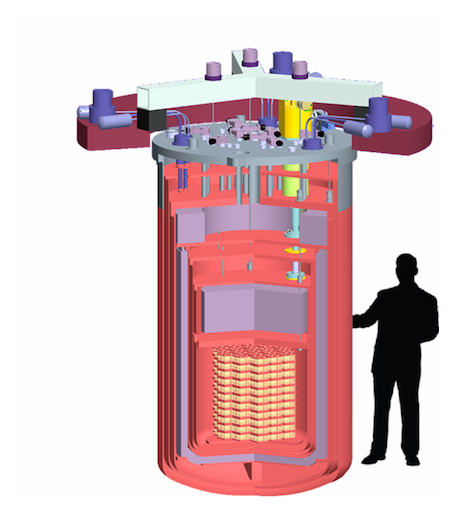
\includegraphics[scale=.8]{img/cuore.eps}
\end{center}
\caption{The CUORE detector and cryostat. In yellow, the 19 towers of bolometers; the lavender volumes are the lead shielding.}\label{fig:cuore}
\end{figure}
%%%%%

The total mass of the detector will be 741 kg for a $^{130}$Te mass of 206 kg. The energy released in a single particle interaction within the crystal is measurable as a change in temperature by  Neutron Transmutation Doped (NTD) germanium thermistors. The measured energy resolution is $\sim 5$ keV FWHM at the $\beta \beta \; (0\nu)$ transition energy ($\sim 2.53$ MeV).

The CUORE bolometers will operate at temperatures between 10 and 15 mK. A challenging $^3$He/$^4$He dilution refrigerator, with a cooling power of 3 mW at 120 mK, has been designed on purpose and is under construction.

A single tower of CUORE, CUORE-0, is presently under construction and will begin  operations within 2011. It will be hosted in the old Cuoricino dilution refrigerator, placed in the hall A of the LNGS. CUORE-0 is a real test of the CUORE assembly chain and procedure, will directly test the level of backgrounds of the CUORE setup and improve the Cuoricino sensitivity on \bbonu.

The CUORE setup will possibly allow in the long term for powerful upgrades. An obvious, though expensive, possibility is to substitute the natural tellurium bolometers with enriched $^{130}$Te units (provided that the enrichment procedure can keep the internal backgrounds very low). A more sophisticated option is to use scintillating crystals containing interesting double beta emitters \cite{Pirro:2005ar}. The contemporary read-out of scintillation light and thermal signal could indeed allow for a dramatic reduction of the background rate and a better characterization of the signal. An array of ZnSe scintillating bolometers, LUCIFER, has been recently proposed as a prototype experiment exploring the performances of such an approach \cite{Ferroni:2011zz} (see sect.~\ref{subsec:other}).




% \subsection{nEXO} \label{subsec:exo}
% %The Enriched Xenon Observatory \cite{Hall:2010zzg} will search for \bbonu\ in \XE. The ultimate goal of the Collaboration is the development of the barium tagging for a multi-ton xenon-based detector, which would lead to a virtually background-free experiment. Prior to that, the Collaboration has built the EXO-200 detector, a $\sim$200-kg liquid xenon (enriched to 80.6\% in \XE) time projection chamber that detects both scintillation and ionization.
%
%The fiducial volume of the chamber, 44 cm in length, is divided in two halves by a central cathode (see fig.~\ref{fig:exo}, left). Ionization charges created in the xenon by charged particles drift under the influence of an electric field towards the two ends of the chamber. There, the charge is collected by a pair of crossed wire planes which measure its amplitude and transverse coordinates. Each end of the chamber includes also an array of avalanche photodiodes (APDs) to detect the 178-nm scintillation light produced by primary interactions. The sides of the chamber are covered with teflon sheets that act as VUV reflectors, improving the light collection. The simultaneous measurement of both the ionization charge and scintillation light of the event may in principle allow to reach a detector energy resolution as low as 3.3\% FWHM at the \XE\ Q-value, for a sufficiently intense drift electric field \cite{EXO-200:2003bso}. 
%
%The xenon is held inside a thin copper vessel immersed in a cryofluid that also shields the experiment from external radioactive backgrounds. The HFE heat-transfer fluid is stored in a vacuum-insulated low-activity copper cryostat. The cryostat is surrounded on all sides by 25 cm of low-activity lead. The entire assembly is surrounded by a radon-free tent and housed in a class 100 clean room, the exterior of which is instrumented on five sides with plastic scintillator panels for vetoing cosmic rays with 95.9\% efficiency. The detector is located 2150 feet underground for an overburden of 1585 meters water equivalent, at WIPP (Waste Isolation Pilot Plant), in the United States.
%
%%%%%%
%\begin{figure}[t!]
%\begin{center}
%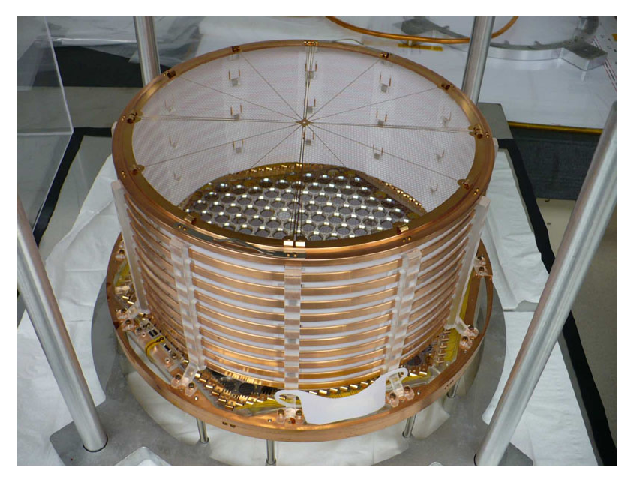
\includegraphics[width=0.475\textwidth]{img/exo1.eps}
%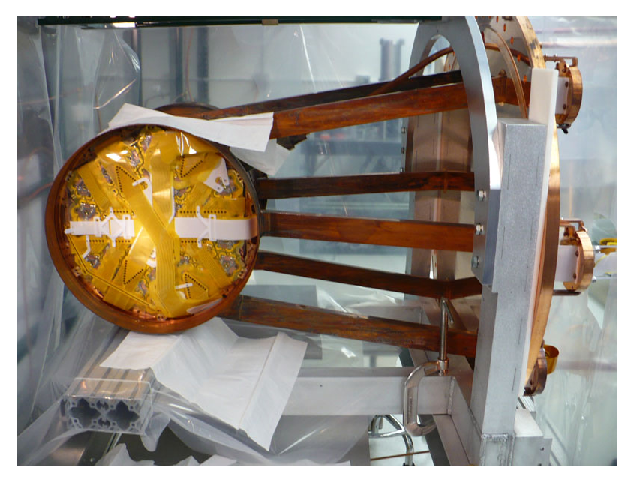
\includegraphics[width=0.475\textwidth]{img/exo2.eps}
%\end{center}
%\caption{Left: one half of the EXO chamber, viewed from the cathode plane. Right: the chamber attached to the cryostat door, as viewed from the bottom of the APD plane. The legs contain the readout cabling and are also the conduits for xenon circulation.} \label{fig:exo}
%\end{figure}
%%%%%%
%
%The EXO-200 TPC was installed in its cryostat in early 2010. The detector was first filled with natural (unenriched) xenon in late 2010. The data collected during these engineering runs were used to make a first assessment of the performance of the detector, and to perform a first round of calibrations. Low-background running with enriched xenon started in the spring of 2011. The EXO Collaboration announced the observation of the \bbtnu\ mode of \XE\ in August 2011. Prior to this measurement, reported in table~\ref{tab:bb2nu_exp}, the \bbtnu\ had been observed in all other important \bbonu\ candidate nuclei except \XE . The measured \bbtnu\ half-life is significantly lower than previously reported lower limits \cite{Bernabei:2002bn,Gavriljuk:2005xc}.
%
%To identify the daughter barium, several methods are under study, including single-ion fluorescence, resonant ionization spectroscopy (RIS), and mass spectroscopy. Single ion fluorescence is a highly sensitive and highly selective method to observe a barium ion while held under vacuum in a RF trap. In this technique, the Ba$^+$ ion is rapidly cycled from its $6^2\text{S}_{1/2}$ ground state to its $6^2\text{P}_{1/2}$ excited state by illuminating it with lasers of the appropriate wavelength (493 nm and 650 nm), see fig.~\ref{fig:bariumenergylevels}. As the electronic state changes, the laser photons are scattered in all directions, and the scattered light can be easily detected by a photo-multiplier tube. EXO has achieved good single barium ion identification with this technique, even in the presence of low pressure xenon and helium gas mixtures. However, this technique also requires that the barium ion be retrieved from the TPC volume, transported to the RF trap, released, and trapped, while not altering its chemical or ionization state. Resonant ionization spectroscopy, on the other hand, is a technique which allows single barium ions to be observed without requiring a vacuum ion trap. In RIS, barium ions are desorbed from the surface of a transport probe, and subsequently resonantly ionized under illumination by 554 nm and 390 nm lasers. The ionized barium can then be observed with a Channeltron electron multiplier. Initial tests with the RIS technique have successfully identified barium being desorbed from the probe tip, so this technique is promising. Other avenues of research include barium identification within xenon ice, and barium extraction from a high pressure gas TPC using gas nozzles. 
% 


The nEXO neutrinoless double beta decay experiment is designed to use a time projection chamber and 5000 kg of isotopically enriched liquid xenon to search for the decay in 136Xe. This detector will be based on very successful EXO-200 detector. A single-phase liquid xenon TPC instrumented to read both scintillation and charge. The anti-correlation of these two signals allowed for an energy resolution of 2.89\% FWHM@Qbb \cite{EXO-200:2020wmu}.

This design also provided the capability of a good fidutialization of the events in the detector and, more important, certain capability to separate them by topology. In particular, the separation of single-site and multi-site events [cite] provided a strong background suppression.

The nEXO design aims to build a volume of 5 tonnes of enriched Xe136. The TPC vessel is a right copper cylinder with both inner height and diameter equal to 127.7 cm surrounded by 33,000 kg of HFE-7000, which serves as both thermal bath and radiation shield. A vacuum layer between an inner vessel and an outer vessel of the cryostat provides thermal insulation from an active water shield, referred to as the outer detector. The TPC itself will have 113.3 cm diameter by 118.3 cm drift height, creating a total xenon mass in the drift region of 3648 kg for an active mass of 3281 kg. This design requires 10 ms of electron life-time to guarantee good energy resolution when reading the ionisation signal. This is achieve by a good purification system and a relatively moderate drift field of 400 V/cm. \cite{nEXO:2021ujk}.



%%%%%%
\begin{figure}[t!]
\begin{center}
\includegraphics[width=0.475\textwidth]{img/nexo_design}
\includegraphics[width=0.475\textwidth]{img/nexo_sipms}
\end{center}
\caption{Left: Close up view of the main components inside the nEXO TPC vessel. Right: Test array of 24 SiPMs used to be used together with charge collection tiles in LXe.Each SiPM is cm$^2$.} \label{fig:nexo}
\end{figure}

Efficient scintillation light collection is an essential requisite for nEXO to attain proper energy resolution and to provide the start time to localize events along the drift field. Actually, in order to reach <2.35\% FWHM energy resolution, the overall optical efficiency must be 3\%  or higher, this is achieved by using SiPMs arrays operated directly in the liquid xenon behind the TPC field shaping rings. The SiPM will have ~1cm$^2$ active area and will be mounted in 24 long staves surrounding the TPC field cage. The necessity of reading as much light as possible has a relevant impact on the TPC design. In particular, the field cage must be as transparent as possible allowing the photons to reach the photsensors region. This affect the geometry of the rings, as they need to be thiner. Also, a coating of vacuum deposited aluminum, protected against oxidation by a layer of MgF2 will make all rings reflective to VUV. In addition, it will allow to remove the traditional PTFE reflective panels used in other liquid xenon TPCs, thus reducing the amount of materials and outgassing inside the detector volume.

One of the main tools the nEXO collaboration proposes to reduce the level of background events is the based on taking advantage of the relatively short attenuation length of $\gamma$-ray at 2.4 MeV energy in LXe, of only 8.7 cm. By selecting a region in the most inner part of the detector they can further reduce the background rate by almost an order of magnitude in the most inner ton of active material. Adding this technique to the energy resolution and topological separation nEXO is predicted to achieve a background rate of 3.6 × 10$^{-4}$ cts/(FWHM·kg·y) in the inner 2000 kg of LXe. 

With this level of background nEXO aims to reach a sensitivity of 9.2 × 10$^{27}$ yrs at 90\% C.L. after 10 years of operation and, an expected 3 sigma discovery potential of 5.7 × 
10$^{27}$ yrs \cite{nexocprecdr}. However, in a recent document \cite{nEXO:2021ujk} the nEXO Collaboration claims for an improved design and understanding of the nEXO design, together with the development of a \bbonu\ DNN discriminator that pushes the background index to 
b=7×10$^{-5}$ cts/(FWHM·kg·yr) obtaining a half-life sensitivity of 1.35×10$^{28}$ 
yr at 90\% C.L.

% \subsection{GERDA} \label{subsec:gerda}
% The GERmanium Detector Array (GERDA) experiment \cite{Abt:2004yk}, located in Hall A of the Laboratori Nazionali del Gran Sasso (LNGS), will make use of naked Ge detectors immersed in a large cryostat of ultra-pure LAr.

The Ge detectors are organized in strings (2--5 detectors) and mounted in special low-mass ($\sim 80$ g) holders made of ultra-pure copper and PTFE. The array of strings is contained in a vacuum insulated stainless steel cryostat of 4.2 m diameter and 8.9 m height. A copper shield covers the inner cylindrical shell of the cryostat with a maximum thickness of 6 cm. The cryostat is placed in a water tank, of 10 m diameter and 9.4 m height, serving as a gamma and neutron shield. It will be also used as a veto against cosmic rays thanks to its instrumentation with 66 photomultipliers, with good efficiency in detecting the Cherenkov light. The cosmic muon veto is reinforced by plastic scintillator panels on top of the detector, for a surface of about 20 m$^2$. A drawing of the detector and shielding is shown in fig.~\ref{fig:gerda}.

%%%%%
\begin{figure}[t!]
\begin{center}
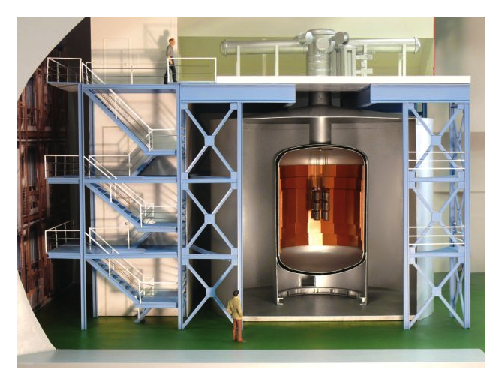
\includegraphics[]{img/gerda.eps}
\end{center}
\caption{Sketch of the GERDA experiment. The germanium arrays can be seen inside the copper cryostat, and this one placed inside the cylindrical water tank.} \label{fig:gerda}
\end{figure}
%%%%%

In its first phase, GERDA-1, eight fully refurbished germanium diodes (17.7 kg total active mass, 86\% isotopic enrichment in \GE ) from the previous Heidelberg-Moscow and IGEX experiments will be used. In the subsequent step, GERDA-2, new diodes will be used for a total active mass of 35.4 kg. These new diodes will be p-type Broad Energy (BEGe) detectors \cite{Budjas:2008wb,Agostini:2010ke}, allowing for a better discrimination of backgrounds thanks to a sophisticated pulse shape discrimination.

The experiment started commissioning runs in June 2010 using natural Ge, low-background, detectors, refurbished from the Genius-TF experiment. These commissioning runs focused on the investigation of the background sources (most notably on the unexpectedly large contribution from $^{42}$Ar-$^{42}$K in the LAr) and on $^{42}$Ar background mitigation strategies, see sect.~\ref{subsec:sensi_assumptions}. Data taking for the GERDA-1 physics run will start in the next months. The background level of the natural Ge setup was measured to be $0.06\pm 0.02$ \ckky\ (corresponding to $0.07\pm 0.02$ \ckkbby ), consistent with early indications from the first string of enriched Ge detectors deployed \cite{Cattadori:2012fy}. This rate, obtained without using pulse shape information, is a factor of 3--4 lower than the HM and IGEX measured ones (see sect.~\ref{subsec:past}), but still about a factor of 6 higher than the GERDA-1 goal. The reason for this higher than expected background rate is at present not fully understood. The goals of GERDA-2 are to start data taking in about two years, with about twice the isotope mass of GERDA-1, and with a background level of 0.001 \ckky\ (or 0.0012 \ckkbby ).

In the very long term a third phase of the experiment, GERDA-3, is foreseen to make use of about 1 ton of $^{76}$Ge target material together with a further reduction of background. Such an effort, common with the MAJORANA project (see below), would be feasible only in a word-wide collaboration, and provided that the GERDA approach could demonstrate to be the best candidate technology to push the double beta decay sensitivity below the inverted hierarchy mass threshold (about 30 meV). 
 

% \subsection{MAJORANA} \label{subsec:majorana}
% The MAJORANA Collaboration is following a more classic approach than GERDA in the design of a germanium-based experiment \cite{Majorana:2011rit}. The Ge detectors will be mounted in a string-like arrangement in ultra-pure vacuum cryostat made from radiopure copper. The cryostat will be surrounded by a passive shielding of Cu and Pb, and an active muon veto.

The Collaboration is building a demonstrator module, to be placed at the Deep Underground Science and Engineering Laboratory (DUSEL) in the United States, with about 20 kg of natural BEGe detectors. The goal is to demonstrate a background rate of about 4 counts per tonne and per year in the 4-keV wide region of interest \cite{Majorana:2011vap}. The demonstrator is expected to operate with enriched detectors in 2013.
 

% \subsection{KamLAND-Zen} \label{subsec:kamland}
% %The KamLAND-Zen experiment will search for \bbonu\ in \XE\ using enriched xenon dissolved in liquid scintillator. This will allow a calorimetric measurement of the \bb\ electrons, as first proposed in \cite{Raghavan:1994qw}. Xenon is relatively easy to dissolve (with a mass fraction of more than 3\% being possible) and also easy to extract from the scintillator. 

%The major modification to the existing KamLAND detector \cite{KamLAND:2002uet} was the construction of an inner, very radiopure (of order $3\times 10^{-12}$ g/g of \URANIUM\ and \THORIUM) and very transparent balloon to hold the dissolved xenon. This balloon, 1.58 m in radius, is placed at the center of the KamLAND active volume as shown in fig.~\ref{fig:kamlandzen}.

%%%%%
%\begin{figure}[t!]
%\begin{center}
%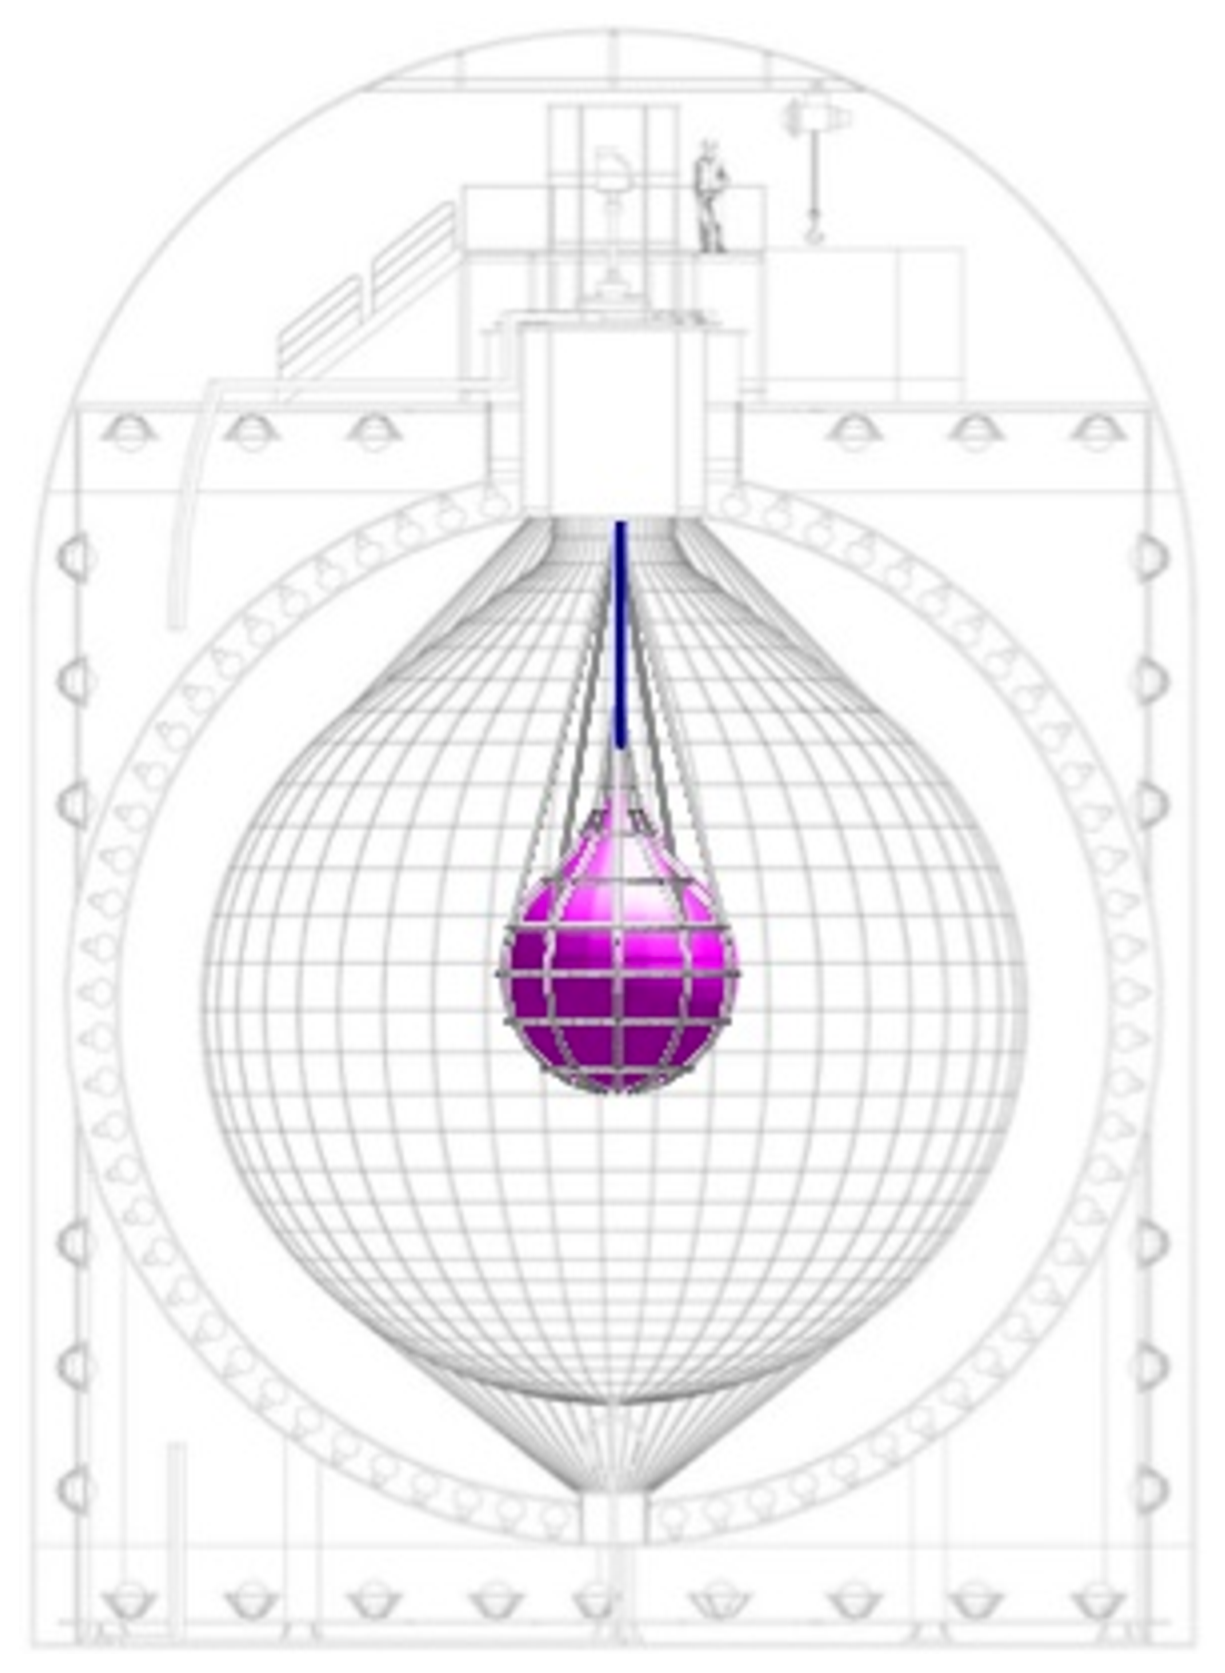
\includegraphics[scale=0.25]{img/kamlandzen.eps}
%\end{center}
%\caption{Sketch of the KamLAND-Zen detector. The ball-on containing the dissolved xenon (purple) hangs in the center of the active volume.} %\label{fig:kamlandzen}
%\end{figure}
%%%%%%

%The KamLAND-Zen experiment plans to dissolve 389 kg of \XE\ in the liquid scintillator of KamLAND in the first phase of the experiment, and up to 1 ton in a projected second phase. 

%The proven resolution (from the previous operation of the KamLAND experiment) is 16\% FWHM at 1 MeV. The main sources of expected background are the \bbtnu\ tail, \BI\ impurities in the scintillator or in the balloon, $^{10}$C generated in the scintillator by cosmic rays, and $^{8}$B solar neutrinos. The expected background rate in the region of interest is $2\times10^{-4}$ \ckky\ \cite{kozlov2011status}, corresponding to $2.2\times10^{-4}$ \ckkbby .

%At the time of writing this report, the mini-balloon installation into the KamLAND detector has been completed, and detector commissioning is ongoing. Physics data-taking with the xenon-loaded liquid scintillator is expected to start in the fall of 2011.



%--------------------------------------------


The KamLAND-Zen experiment is a neutrinoless double beta decay search conducted using the KamLAND detector, a liquid scintillator-based neutrino detector located in the Kamioka mine in Japan. The experiment utilises a large volume of liquid scintillator, doped with a high concentration of Xenon enriched in the Xe136 isotope to enhance the sensitivity to neutrinoless double beta decay.

The KamLAND-Zen detector re-uses the KamLand facility, a spherical volume filled with approximately 1000 tons of liquid scintillator. This volume, designed originally to detect MeV neutrinos, have a very low concentration of $^{238}$U and $^{232}$Th, at the level of 5.0x10$^{-18}$ and 1.3x10$^{-17}$ respectively and it is used in Kamland-Zen as active veto. At the center of this volume, a smaller balloon made out of ethylene-vinylalcohol co-polymer and nylon with a 6.5 m radius and 135 $\mu$m thickness defines a different scintillating volume with xenon dissolve in it. This design allows for accumulation of large amounts of isotope in a very clean environment, the detector configuration also allows to reconstruct the position of the events, allowing to select events far from the ballon walls.
On the other hand as the measurement is based only on the scintillation light, they lack of a good energy resolution producing relatively large background rates in their region of interest when compared with other experiments. In addition, the capabilities of KamLAND-Zen to distinguish among different type of particle interactions is very reduce, although some efforts using neural networks \cite{https://arxiv.org/abs/2203.01870} allow for slightly improved background rejection.
Another issue they face due to their large volume is the relevant contribution to the total background of spallation products that forces to add analysis cuts to select event separated enough in time from muon-induced showers.


%%%%%
\begin{figure}[t!]
\begin{center}
\includegraphics[scale=0.25]{img/KL_fidutial}
\includegraphics[scale=0.25]{img/KL_LD_events}
\end{center}
\caption{Top:Vertex distribution of candidate events (black points) overlaid on $^{214}$Bi background events from the MC simulation (color histogram) in the energy region 2.35 < E < 2.70 MeV (\bbonu\ window), with arbitrary normalization. The solid and thick dashed lines indicate the shape of the IB and the 1.57-m-radius spherical volume, respectively. The dot-dashed line indicates the nylon belt suspending the inner ballon. The thin dashed lines illustrate the shape of the equal-volume spherical half-shells, which compose the 2.5-m-radius spherical fiducial volume. The high-count region at the IB bottom indicates the hot spot and is vetoed.
Bottom:Energy spectra of selected ββ candidates within a 1.57-m-radius spherical volume drawn together with best-fit backgrounds, the 2νββ decay spectrum, and the 90\% C.L. upper limit for \bbonu\ decay of  long-lived data (LD).
} \label{fig:kamlandzen}
\end{figure}
%%%%%%


The current phase of the KamLAND-Zen experiment uses 745 kg of xenon enriched at the 91\% level in the \XE\ isotope \cite{https://arxiv.org/abs/2203.02139}. This is nearly a factor of two in active mass with respect the previous phase of the experiment. The KL collaboration has recently published the results of their last period of data taking \cite{https://arxiv.org/abs/2203.02139} that corresponds to a total exposure of 970 kg yr of \XE\ . Along this period they observe a total of 24 background events, which can be described by the background-dominated approximation. In this analysis they do not find event excess over the expected background setting a limit to the  half-limit in Xe that corresponds to $T_{1/2} > 2.0X10^{26}$ yr (90\% C.L.), even when their sensitivity was 1.3X10$^{26}$. The combined analysis of this data with the KamLAND-Zen 400 pushes further this limit to $T_{1/2} > 2.3X10^{26}$ yr (90\% C.L.), being the best world limit to this process for xenon.
These results set upper limits on the effective Majorana mass of 36-156 meV depending of the NMEs used.


% \subsection{NEXT} \label{subsec:next}
% The Neutrino Experiment with a Xenon TPC (NEXT) \cite{NEXT:2011eyk} will search for \bbonu\ in \XE\ using a 100-kg high-pressure gaseous xenon (HPXe) time projection chamber. 
Such a detector can provide both good energy resolution and event topological information for background rejection \cite{Nygren:2009zz}.

Double beta decay events leave a distinctive topological signature in HPXe: a ionization track, of about 30 cm long at 10 bar, tortuous due to multiple scattering, and with larger energy depositions at both ends (see fig.~\ref{fig:next_track}). The Gotthard experiment \cite{Luscher:1998sd}, consisting in a small xenon TPC (5.3 kg of xenon, 68\% enrichment in \XE ) operated at 5 bar, proved the effectiveness of such a signature to reject background, achieving a background rate of only $\sim0.01$ \ckky.

%%%%%
\begin{figure}[t!]
\vspace{0.75cm}
\begin{center}
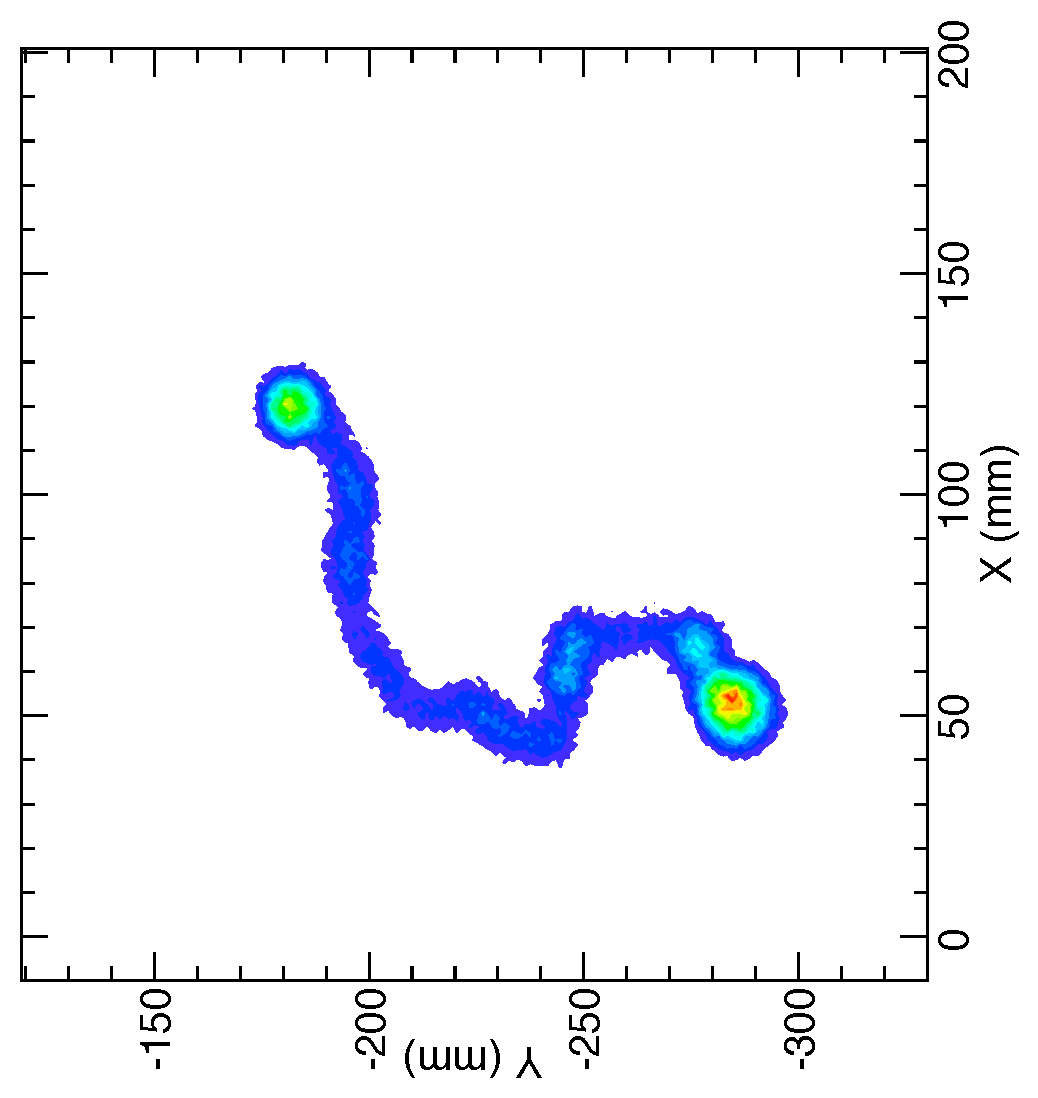
\includegraphics[angle=-90,scale=0.45]{img/bb0nu_track_10atm.eps}
\end{center}
\caption{Simulation of a \bbonu\ track in gaseous xenon at 10 bar \cite{NEXT:2011eyk}.} \label{fig:next_track}
\end{figure}
%%%%%

The design of NEXT is optimized for energy resolution (better than 1\% FWHM at $Q_{\beta \beta}$) by using proportional electroluminescent (EL) amplification of the ionization signal. The detection process is as follows. Particles interacting in the HPXe transfer their energy to the medium through ionization and excitation. The excitation energy is manifested in the prompt emission of VUV ($\sim$178 nm) scintillation light. The ionization tracks (positive ions and free electrons) left behind by the particle are prevented from recombination by a strong electric field (0.5--1.0 kV/cm). Negative charge carriers drift toward the TPC anode, entering a region, defined by two highly-transparent meshes, with an even more intense electric field (3.5 kV/cm/bar). There, further VUV photons are generated isotropically by electroluminescence. Therefore, both scintillation and ionization produce an optical signal, to be detected with a sparse plane of PMTs located behind the cathode. The detection of the primary scintillation light constitutes the start-of-event ($t_0$), whereas the detection of EL light provides an energy measurement. Electroluminescent light provides tracking as well, since it is detected also a few mm away from production at the anode plane, via a dense array (1 cm pitch) of 1-mm$^{2}$ SiPMs.

The NEXT detector will operate at 10 bar, with xenon enriched at 90\% in the \XE\ isotope. At that pressure the 100 kg mass of xenon results in a volume of $\sim$2.5 m$^3$.

The major benefits of the NEXT 100 proposal are its high background rejection factor, resulting in an expected background rate of $2\times 10^{-4}$ \ckkbby , and the fact that xenon is relatively easy (cheap) to enrich and obtain in large quantities.

The NEXT Collaboration expects to commission the detector at the end of 2013. The experiment plans to start its physics run in the second half of 2014.


% \subsection{SNO+} \label{subsec:sno+}
% SNO+ \cite{Kraus:2010zzb} is the follow-up of the successful SNO experiment \cite{SNO:1999crp}, located at SNOLAB, in Canada. It re-uses the existing equipment of the detector (acrylic vessel, photomultipliers and their support structure, electronics and the light water shield) replacing the heavy water by $\sim$780 tonnes of liquid scintillator (linear alkylbenzene, LAB).

The physics program of the SNO+ detector includes measurements of low energy solar neutrinos and \bbonu\ searches using \ND. In order to do that, the liquid scintillator will be loaded with a neodymium salt, resulting in about 50 kg of \ND. This isotope has the second highest endpoint, 3.37 MeV, and the fastest predicted neutrinoless double beta decay rate due to its large phase space factor, see fig.~\ref{fig:g0nu}. The high endpoint is above most radioactive backgrounds, such as radon, and this is a significant advantage. However, enrichment of this isotope seems difficult.

The energy resolution of the SNO+ detector is estimated to be 6.5\% FWHM at 3.4 MeV. External backgrounds can be rejected with a relatively tight fiducial volume selection, cutting however about 50\% of the signal. The most important sources of background are expected to be \TL\ impurities in the scintillator, the irreducible background from $^{8}$B solar neutrinos and \bbtnuº events from \ND . Assuming the radiopurity levels for the liquid scintillator achieved by BOREXINO ($\sim10^{-17}$ g/g of \TL) \cite{Borexino:2009awt}, simulations predict a background rate of $\sim10^{-2}$ \ckkbby\ \cite{Wright:2009csa}. 

The SNO+ experiment is expected to start commissioning in the spring of 2013 with pure liquid scintillator, to be followed by the Nd-loaded liquid scintillator phase. Given that the LAB liquid scintillator is about 15\%  less dense than the surrounding light water, one of the major technical challenges of the SNO+ upgrade is the design of a hold-down system for the acrylic vessel using a net of radiopure ropes, see fig.~\ref{fig:snoplus_anchor_possibility}.  

%%%%%
\begin{figure}[t!b!]
\begin{center}
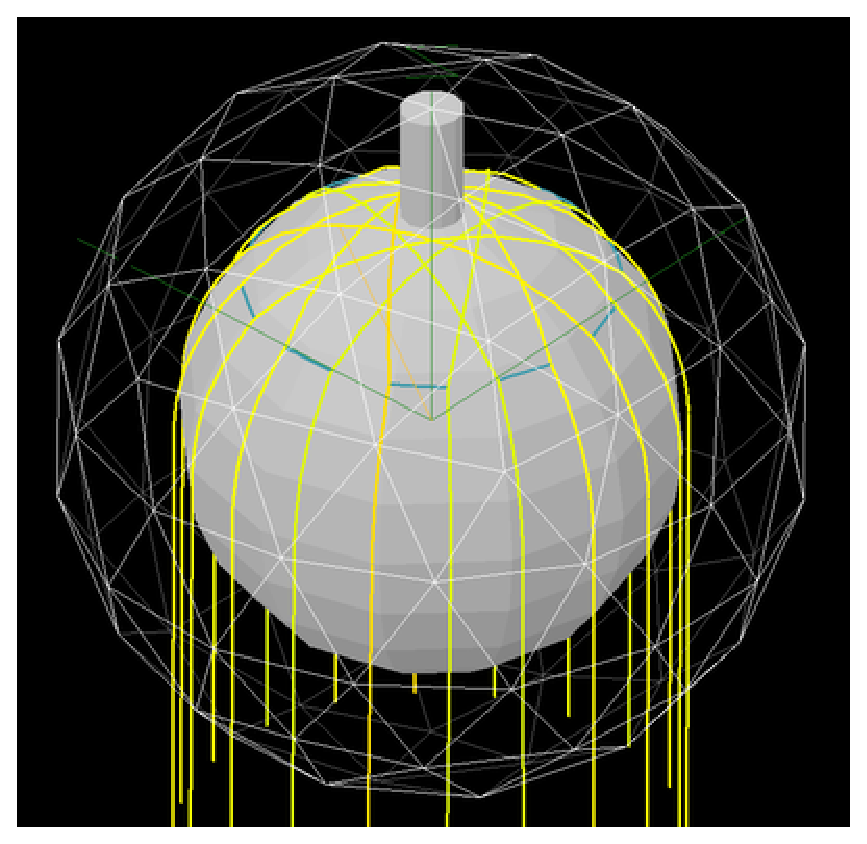
\includegraphics[width=0.55\textwidth]{img/Snoplus_anchor_possibility.eps}
\end{center}
\caption{\label{fig:snoplus_anchor_possibility}One of the candidate configurations for the SNO+ acrylic vessel anchor system. The acrylic vessel is shown in grey, and the anchor system in yellow. The outer sphere made of triangles is the PMT support structure.} 
\end{figure}
%%%%%

% \subsection{SuperNEMO} \label{subsec:snemo}
% This proposed new installment of the NEMO detectors series consists of up to 20 tracker-calo modules, each one containing a thin foil of about 5 kg of \bb-decaying material, probably \SE, although other isotopes such as \ND\ or \CA\ are also under consideration. 

A sketch of a SuperNEMO module can be seen in fig.~\ref{fig:snemo}. The source foil, 3 meters high and 4.5 meters long, with a surface density of about 40 mg/cm$^{2}$, is placed in the center of a tracking chamber with overall dimensions of 4 m height, 5 m length and 1 m width. Nine planes of drift cells operating in Geiger mode and a magnetic field of 25 Gauss allow to reconstruct the trajectory and charge of particles crossing the chamber. A calorimeter consisting of blocks of plastic scintillator coupled to low-activity PMTs surrounds the tracking chamber on four sides. Its granularity allows the energy of individual particles to be measured.

%%%%%
\begin{figure}[t!b!]
\begin{center}
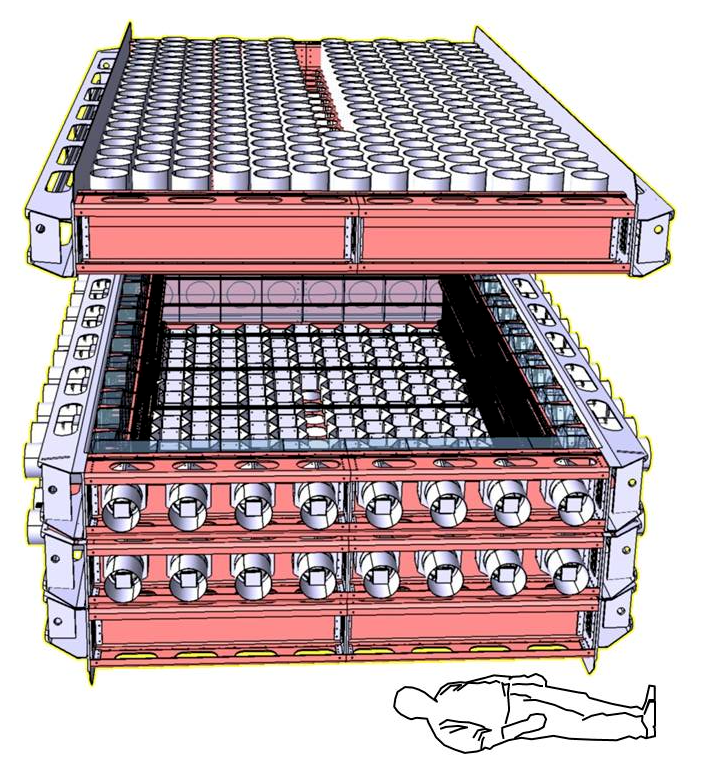
\includegraphics[angle=270,width=0.45\textwidth]{img/snemo-1.eps} \hspace{0.04\textwidth}
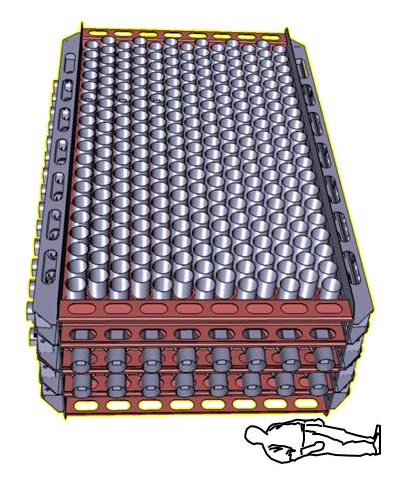
\includegraphics[angle=270,width=0.45\textwidth]{img/snemo-2.eps}
\end{center}
\caption{A SuperNEMO module. The source foil (not shown) is placed in the center of a tracking volume consisting of drift cells operating in Geiger mode. The tracking volume is surrounded by calorimetry consisting of scintillator blocks connected to PMTs (grey). The support frame is shown in red.} \label{fig:snemo}
\end{figure}
%%%%%

The physics case of SuperNEMO relies on several significant improvements over the NEMO-3 detector performance \cite{Shitov:2010nt}. The energy resolution is expected to be 7\% FWHM at 1 MeV, a factor of 2 better than in NEMO-3. Such a resolution has been attained with a 28 cm hexagonal PVT scintillator directly coupled to a 8-inch PMT \cite{Freshville:2011zz}. The detection efficiency of SuperNEMO is estimated by means of simulation to be about 30\%, almost a factor of 2 better than in NEMO-3. As far as the backgrounds are concerned, SuperNEMO goals require an impressive improvement in the purification (both chemical and via distillation methods) of the source foils. In particular, \BI\ and \TL\ contamination in \SE\ foils are to be reduced by factors of 50 and 170, respectively. A dedicated setup, the BiPo detector, installed in the Laboratorio Subterr\'aneo de Canfranc (LSC), will measure the radiopurity of the foils in order to make sure that the required levels are achieved. Finally, in order to decrease radon gas levels in the tracking chamber down to negligible levels ($<$0.15 mBq/m$^3$ ), a reduction of at least a factor of 40 with respect to NEMO-3 is needed. 

The first SuperNEMO module, called the demonstrator, will be the first step from R\&D to construction with the aims to demonstrate the feasibility of large scale mass production, to measure the backgrounds (especially from radon emanation), and to finalize the detector design. The demonstrator will be installed in the space previously occupied by the NEMO-3 detector at the Modane Underground Laboratory.

The current plans of the SuperNEMO Collaboration for the following: (a) demonstrator construction, 2010--2012; (b) demonstrator physics run start-up, 2013; and (c) full detector construction start-up, 2014. 

% \subsection{Other proposals} \label{subsec:other}
% \subsubsection*{CANDLES} This project \cite{Umehara:2010zz} proposes the use of CaF$_{2}$ scintillating crystals to search for \bbonu\ in \CA. The crystals would be immersed in liquid scintillator providing shielding and an active veto against external backgrounds. Among the \bb\ isotopes, \CA\ has the highest $Q$-value, 4.27 MeV. This places the signal well above the energy region of the natural radioactive processes. Unfortunately, the natural abundance of the isotope is only 0.187\% and enrichment seems complicated. Therefore, many tons of crystals are needed for a competitive new-generation experiment.  
%
\subsubsection*{COBRA} The COBRA experiment \cite{Zuber:2001vm, Zuber:2010zz} is exploring the potentials of Cadmium Zinc Telluride (CdZnTe) room-temperature semiconductor detectors for \bbonu\ searches. Out of the several \bb\ candidate isotopes in CdZnTe, COBRA is focusing on \TE, because of its natural abundance, and \CD, because of its high $Q$-value of 2.8 MeV. Activities are split in two main directions: (a) the identification of the main background components in a setup of 64 commercial 1-cm$^{3}$ CdZnTe diodes located at LNGS; and (b) the development of pixelized devices that would allow to reduce the background by particle identification.
%
\subsubsection*{DCBA} The Drift Chamber Beta-ray Analyzer \cite{Ishikawa:2011zza} is a magnetized tracker (drift chambers) that can reconstruct the trajectories of charged particles emitted from a \bb\ source foil. The momentum and kinetic energy are derived from the track curvature in the magnetic field. A prototype, DCBA-T2, has shown energy resolution of about 150 keV (FWHM) at 1 MeV, and the main source of background (\BI) has been identified. A new apparatus, DCBA-T3, with a more intense magnetic field is now under construction at KEK.
%
\subsubsection*{LUCIFER} The idea of LUCIFER \cite{Giuliani:2010zz, Ferroni:2011zz} is to join the bolometric technique proposed for the CUORE experiment with the bolometric light detection technique used in cryogenic dark matter experiments. Preliminary tests on several \bbonu\ detectors have clearly demonstrated the background rejection capabilities that arise from the simultaneous, independent, double readout (heat and scintillation). LUCIFER will consist of an array of ZnSe crystals operated at 20 mK. The proof of principle with about 10 kg of enriched Se is foreseen for 2014.
%
\subsubsection*{MOON} The MOON detector \cite{Ejiri:2010zz} is a stack of multi-layer modules, each one consisting of a scintillator plate for measuring energy and time, two thin detector layers for position and particle identification, and a thin \bb\ source film interleaved between them. At present, NaI(Tl) scintillators are considered as the candidates for the scintillator plates. Energy resolution around 3\% FWHM at 3 MeV has been achieved during the R\&D phase. For position-sensitive detectors, possible candidates are multi-wire proportional chambers (MWPCs) and Si-strip detectors. 
%
\subsubsection*{XMASS} XMASS \cite{Sekiya:2010bf, Takeda:2011zza} is a multi-purpose liquid xenon scintillator. Although optimized for dark matter searches, it will also investigate neutrinoless double beta decay and solar neutrinos. The detector, with about 800 kg of xenon, was installed in the Kamioka mine (Japan) in the fall of 2010. The excellent self-shielding capabilities of the liquid xenon will be used to define a virtually background-free inner volume. 
%%%

% \subsection{Sensitivity of new-generation experiments} \label{subsec:sensi}
% In this section we try to assess the physics case of the new-generation double beta experiments described above\footnote{For the sensitivity computation, we restrict ourselves to experiments that involve at least a few kg of \bb\ emitter mass, that are approved, and that have been granted a significant financial support.}. We quote the experimental sensitivities to \mbb, assuming the standard light Majorana neutrino exchange as the dominant \bbonu\ mechanism. To perform this risky exercise we make use of the physics-motivated ranges for the NME values described in sect.~\ref{subsec:nme_pmr}, and of the set of experimental parameters summarized in table~\ref{tab:parameters}. A discussion motivating our choice of parameters in table~\ref{tab:parameters} is given in sect.~\ref{subsec:sensi_assumptions}.

%%%%%
\clearpage
\begin{sidewaystable}[H]
\caption{Basic parameters for the different double beta experiments: \bb\ emitter mass \Mbb, \bbonu\ efficiency $\varepsilon$, FWHM energy resolution $\Delta E$, and background rate $c$ per unit energy, \bb\ isotope mass and time. The last column indicates the number of background events within the ROI, and is the product of the \Mbb, $\Delta E$ and $c$ columns. Comparison of different approaches is very difficult directly from the numbers in the table, but this information is fundamental to compute their sensitivity.}\label{tab:parameters}
\begin{center}
\begin{tabular}{lcccccc}
\hline
Experiment  & \Mbb    & $\varepsilon$ & $\Delta E$ & $c$                  & Bgr/ROI   \\
            & (\kgbb) &               & (keV)      &  ($10^{-3}$ \ckkbby)  & (cts/yr)   \\ \hline
EXO-200     & 141     & 0.34 	      & 100        & 0.78--5              & 11--71  \\
GERDA-1     & 15.2    & 0.95          & 4.2        & 12--70               & 0.77--4.5  \\
GERDA-2     & 30.4    & 0.84          & 2          & 1.2--7               & 0.07--0.43 \\ 
CUORE-0     & 10.9    & 0.83          & 5          & 180--390             & 9.8--21.3  \\
CUORE 	    & 206     & 0.83          & 5    	   & 36--130              & 37.1--134  \\
KamLAND-Zen & 357     & 0.61          & 250 	   & 0.22--1.8            & 19.6--161  \\
MAJORANA Demonstrator   & 17.2    & 0.85          & 2          & 1.2--12              & 0.04--0.41  \\  
SNO+        & 44      & 0.50          & 220        & 9--70                & 87--680 \\
NEXT 	    & 89.2    & 0.33 	      & 18         & 0.2--1               & 0.32--1.6 \\
SuperNEMO Demonstrator  & 7       & 0.28          & 130        & 0.6--6               & 0.55--5.5 \\
 \hline
\end{tabular}
\end{center}
\end{sidewaystable}
%%%%%

Although different experimental aspects are relevant from the point of view of the feasibility of an experiment, the sensitivity can be computed using only a few parameters ---namely, effective mass of the isotope and background rate in the energy Region Of Interest (ROI)--- that can be extracted from the fundamental numbers in the design of the experiments. 

The sensitivity is calculated based on the Feldman-Cousins method \cite{Feldman:1997qc} for constructing confidence intervals, following the prescription given in \cite{Gomez-Cadenas:2010zcc}. For each experiment, we define a ROI centered at the \bb\ decay $Q$-value and extending for one FWHM of energy resolution, and we compute the experimental sensitivity at 90\% confidence level. We take into account the effect of the FWHM selection (corresponding to 76\% efficiency assuming gaussian resolution) as a multiplicative factor to the experimental efficiency reported in table~\ref{tab:parameters}.

 Our prescription assumes a counting experiment in the ROI with a perfectly known background rate. In other words, in our sensitivity computation, we neglect systematic uncertainties\footnote{With one exception for the SNO+ and KamLAND-Zen experiments, see sect.~\ref{subsec:sensi_assumptions}, where an attempt has been made to account for systematic effects affecting energy reconstruction.} and any energy shape information that may be present in the energy distribution of events. Systematic uncertainties may possibly affect the parameters listed above, especially the knowledge of the backgrounds, and deteriorate the sensitivity. On the other hand, use of additional information beyond the overall count rate of \bbonu\ candidates within the ROI may yield some sensitivity improvement. While important, both effects would be extremely difficult to incorporate in such a sensitivity comparison, given that most new-generation experiments discussed here have not even started their commissioning phase, yet.

In fig.~\ref{fig:sens-pmr} we show the \mbb\ sensitivities at 90\% CL for the new-generation proposals discussed above, assuming a 5 years exposure for all of them. The colored rectangles reflect the uncertainty coming from the PMR nuclear matrix elements, see fig.~\ref{fig:nme}. For each experiment, two rectangles are shown, corresponding to the most optimistic and most pessimistic background rate expectations given in tab.~\ref{tab:parameters}, respectively. For most experiments, the two rectangles overlap. For each experiment, the thin solid line at the lowest \mbb\ values is meant to give an idea of what can be gained by increased exposures. The line represents the \mbb\ sensitivity for the most optimistic NME values (within the PMR range of fig.~\ref{fig:nme}) and for the most optimistic background rate expectations (within the ranges of tab.~\ref{tab:parameters}) for a 10 years exposure. For reference, we also show the mass range of the standing KK claim of evidence for \bbonu\ in \GE\ \cite{Klapdor-Kleingrothaus:2006zcr} (with a central value of 300 meV) and the mass region as predicted under the inverted hierarchy hypothesis (between 17 and 52 meV, see fig.~\ref{fig:mbetabetavsmlight}). The sensitivity of the various proposals after a 5 years exposure, both in terms of \Tonu\ and \mbb, is also shown in tab.~\ref{tab:sensitivity}, where the central value of the PMR interval for the nuclear matrix elements and the optimistic background rate expectations in tab.~\ref{tab:parameters} have been assumed.


\begin{figure}[ht]
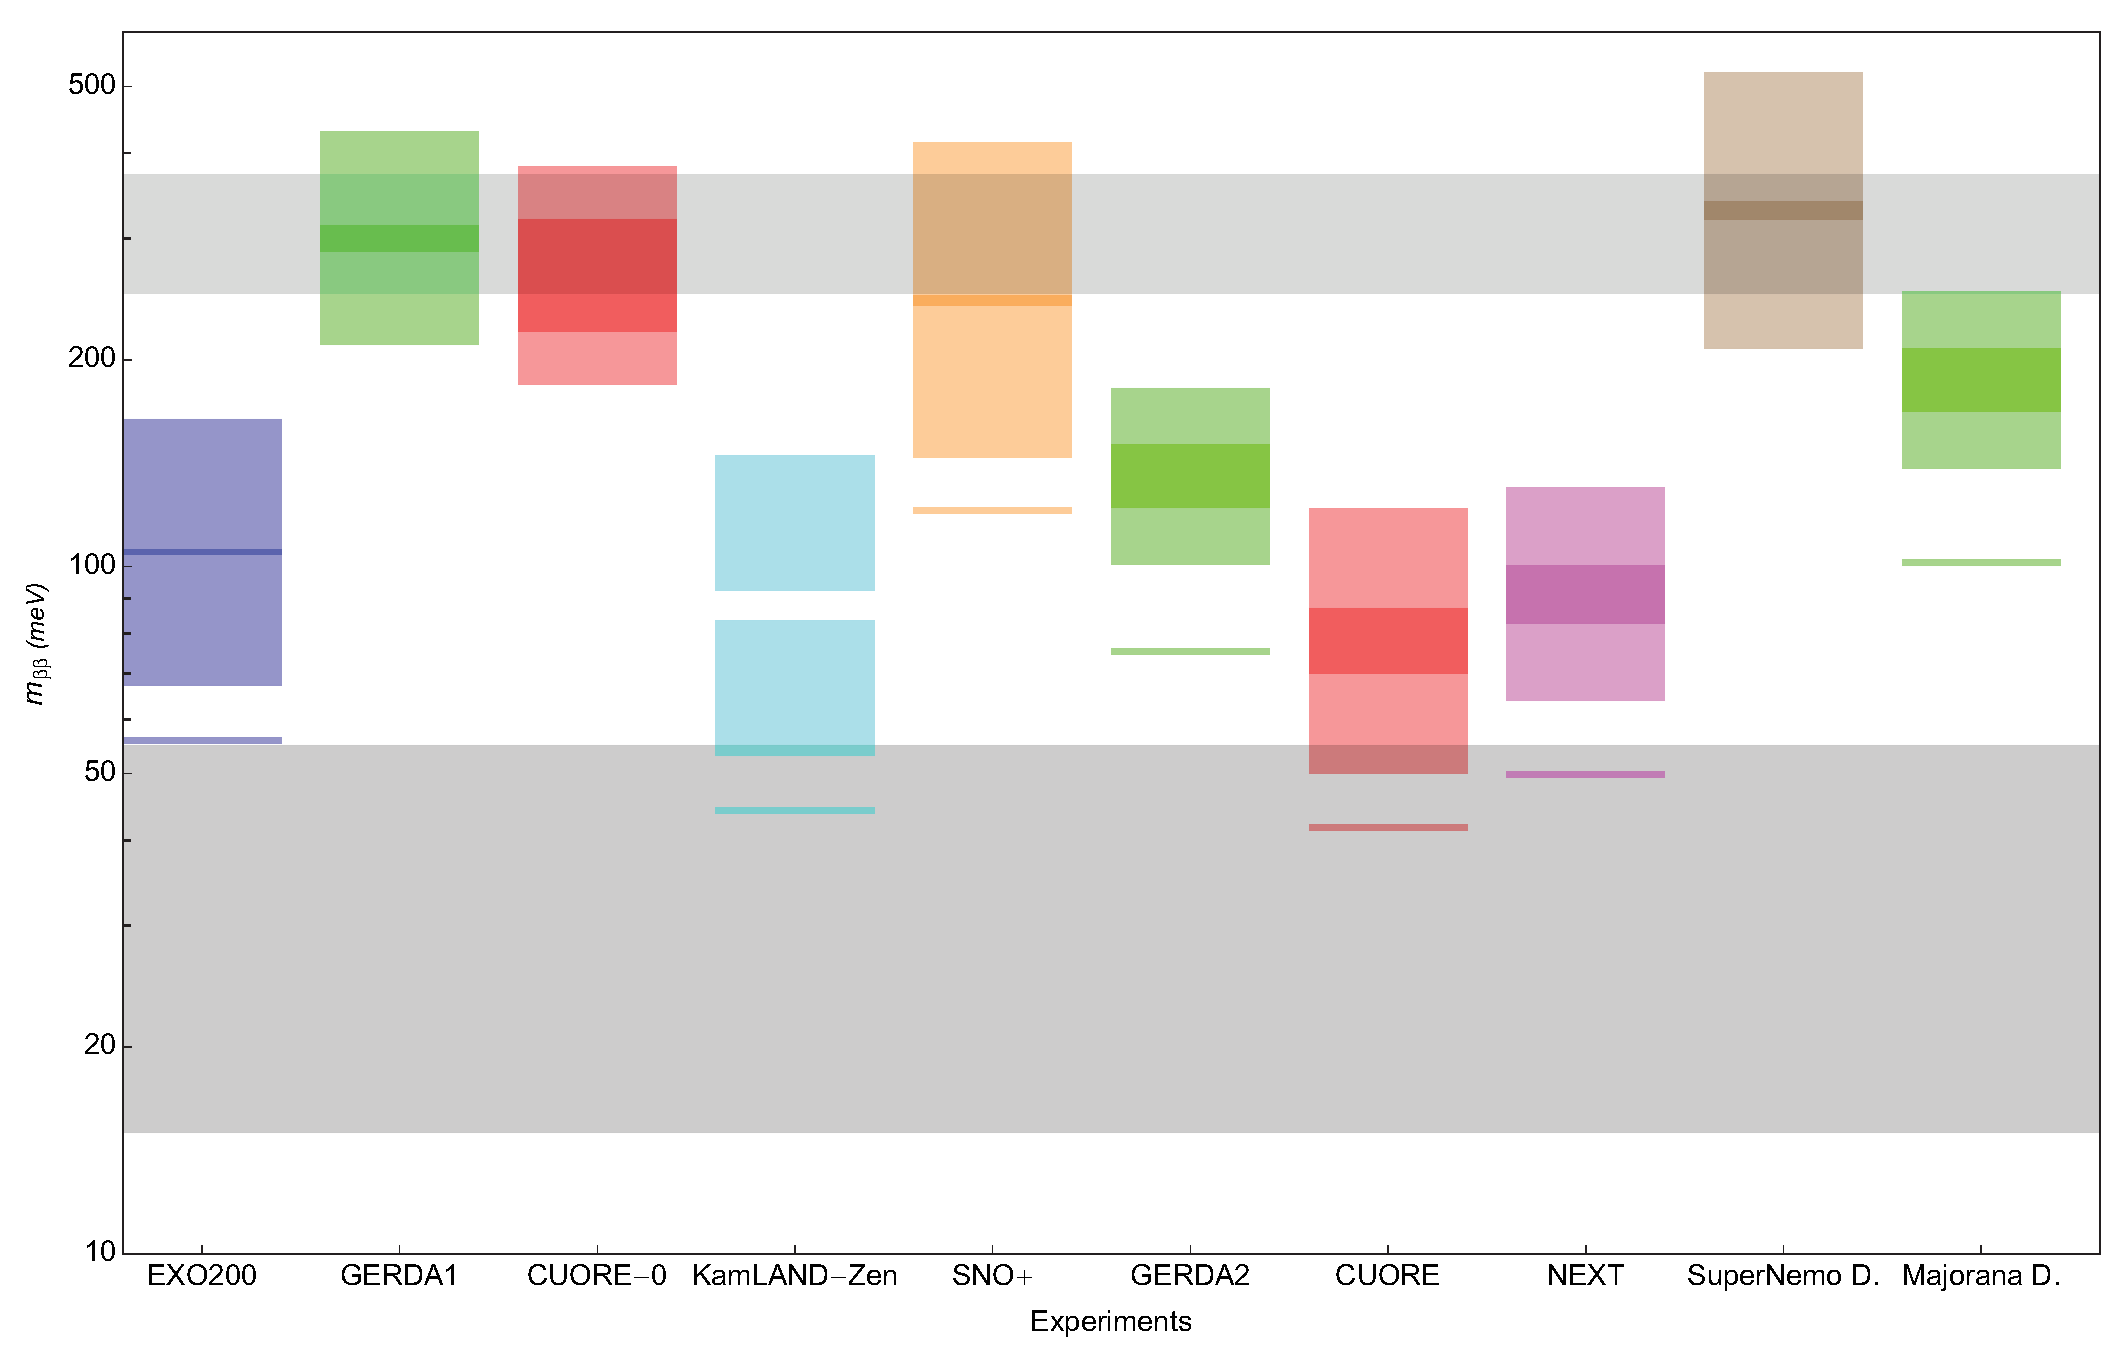
\includegraphics[width=\textwidth]{img/DB_parameters.eps}
\caption{Sensitivity of the different experiments to the neutrino effective mass \mbb\ computed assuming a 5 years exposure, the PMR intervals for the nuclear matrix elements (see sect.~\ref{subsec:nme_pmr}), and for both the optimistic and pessimistic experimental parameters of table~\ref{tab:parameters}. A statistical 90\% CL is computed according to the Feldman-Cousins method \cite{Feldman:1997qc}, assuming a signal region of one FWHM and the corresponding efficiency. For each experiment, the sensitivities for the two experimental parameter sets are drawn as overlapping rectangles. A sensitivity line corresponding to a 10 years exposure, and to the most optimistic NME and experimental parameter set, is also shown. The upper grey region represents the KK claim \cite{Klapdor-Kleingrothaus:2006zcr} while the lower grey region represents the inverted hierarchy region (see fig.~\ref{fig:mbetabetavsmlight}).}
\label{fig:sens-pmr}
\end{figure}


%%%%%
\begin{table}[t!b!]
\caption{Sensitivity of the experiments at 90\% CL after a 5 years exposure, both in terms of half-life \Tonu\ and in terms of neutrino effective mass \mbb . These values are obtained from the optimistic background rate assumptions in tab.~\ref{tab:parameters}. The conversion from \Tonu\ to \mbb\ assumes the central value of the PMR interval for the nuclear matrix elements.}\label{tab:sensitivity}
\begin{center}
%\begin{narrowtabular}{3cm}{lcr}
\begin{tabular}{lcr}
\hline
Experiment & \Tonu\ (years) & \mbb\ (meV) \\ \hline
CUORE-0 	& $8.67\times 10^{24}$ & 203 \\
CUORE 		& $8.86\times 10^{25}$ & 63\\
GERDA-1 	& $4.49\times 10^{25}$ & 252\\
GERDA-2 	& $1.37\times 10^{26}$ & 121\\
EXO200 		& $8.20\times 10^{25}$ & 82\\
NEXT 		& $9.13\times 10^{25}$ & 78\\
KamLAND-Zen 	& $1.32\times 10^{26}$ & 65\\
SNO+ 		& $5.38\times 10^{24}$ & 182\\
SuperNEMO Demonstrator 	& $9.15\times 10^{25}$ & 258\\
MAJORANA Demonstrator	& $7.19\times 10^{25}$ & 258\\
 \hline
%\end{narrowtabular}
\end{tabular}
\end{center}
\end{table}
%%%%%

The first thing to remark from fig.~\ref{fig:sens-pmr} is that the KK claim should be unambiguously solved by several new-generation proposals using different isotopes. If our assumptions are correct, this will certainly be the case for \GE\ (GERDA, MAJORANA), \TE\ (CUORE) and \XE\ (EXO-200, KamLAND-Zen, NEXT), and possibly also for \SE\ (SuperNEMO) and \ND\ (SNO+). Multi-isotope determination of \bbonu\ may therefore become a real possibility within this decade. In this respect, it is important to note that GERDA and MAJORANA are the only experiments among those in fig.~\ref{fig:sens-pmr} using the same isotope of the HM experiment\footnote{Not only: we have seen that GERDA in its first phase re-uses the same detectors as in the HM experiment.}, and should therefore be able to provide the only truly model-independent confirmations of this claim.

On the other hand, several experiments appear to have a very good chance to reach a sensitivity of 100 meV or better, in particular CUORE, KamLAND-Zen, NEXT and EXO-200. In our most optimistic scenario concerning NME values and experimental performances, this target may also be reached by GERDA during its second phase. Given our uncertainties, we cannot predict which, among these 4--5 different experimental proposals, will provide the best \mbb\ sensitivity after a 5 years exposure. To this end, a better knowledge of the actual (as opposed to expected) values for the background rates, of the systematic uncertainties affecting the measurement, and of the NME values would be necessary for all experiments.

From fig.~\ref{fig:sens-pmr}, our expectation is that it will be almost impossible for the new-generation experiments discussed here to discover \bbonu\ after 5 years of exposure if the neutrino mass spectrum is hierarchical ($m_{\rm light}\simeq 0$) rather than degenerate, since essentially no overlap exists between the experimental sensitivities and the 17--52 meV inverted hierarchy region. Not only larger exposures, but also new (better) experimental proposals, would be needed to fully probe this mass region. As mentioned above, we expect experiments using \XE\ (EXO-200, KamLAND-Zen, NEXT) to provide for the first time during this decade a comparable or better sensitivity than \GE\ (GERDA, MAJORANA) and \TE\ (CUORE) experiments, which dominated the field over the past two decades. In perspective, if the low-background expectations of new-generation \XE\ proposals will be confirmed during this decade, \XE\ would be a particularly favorable isotope to use also in the longer term. This is because scalability to isotope masses in the 1-10 ton range are in this case more realistic than with any other isotope. 

\begin{figure}[ht]
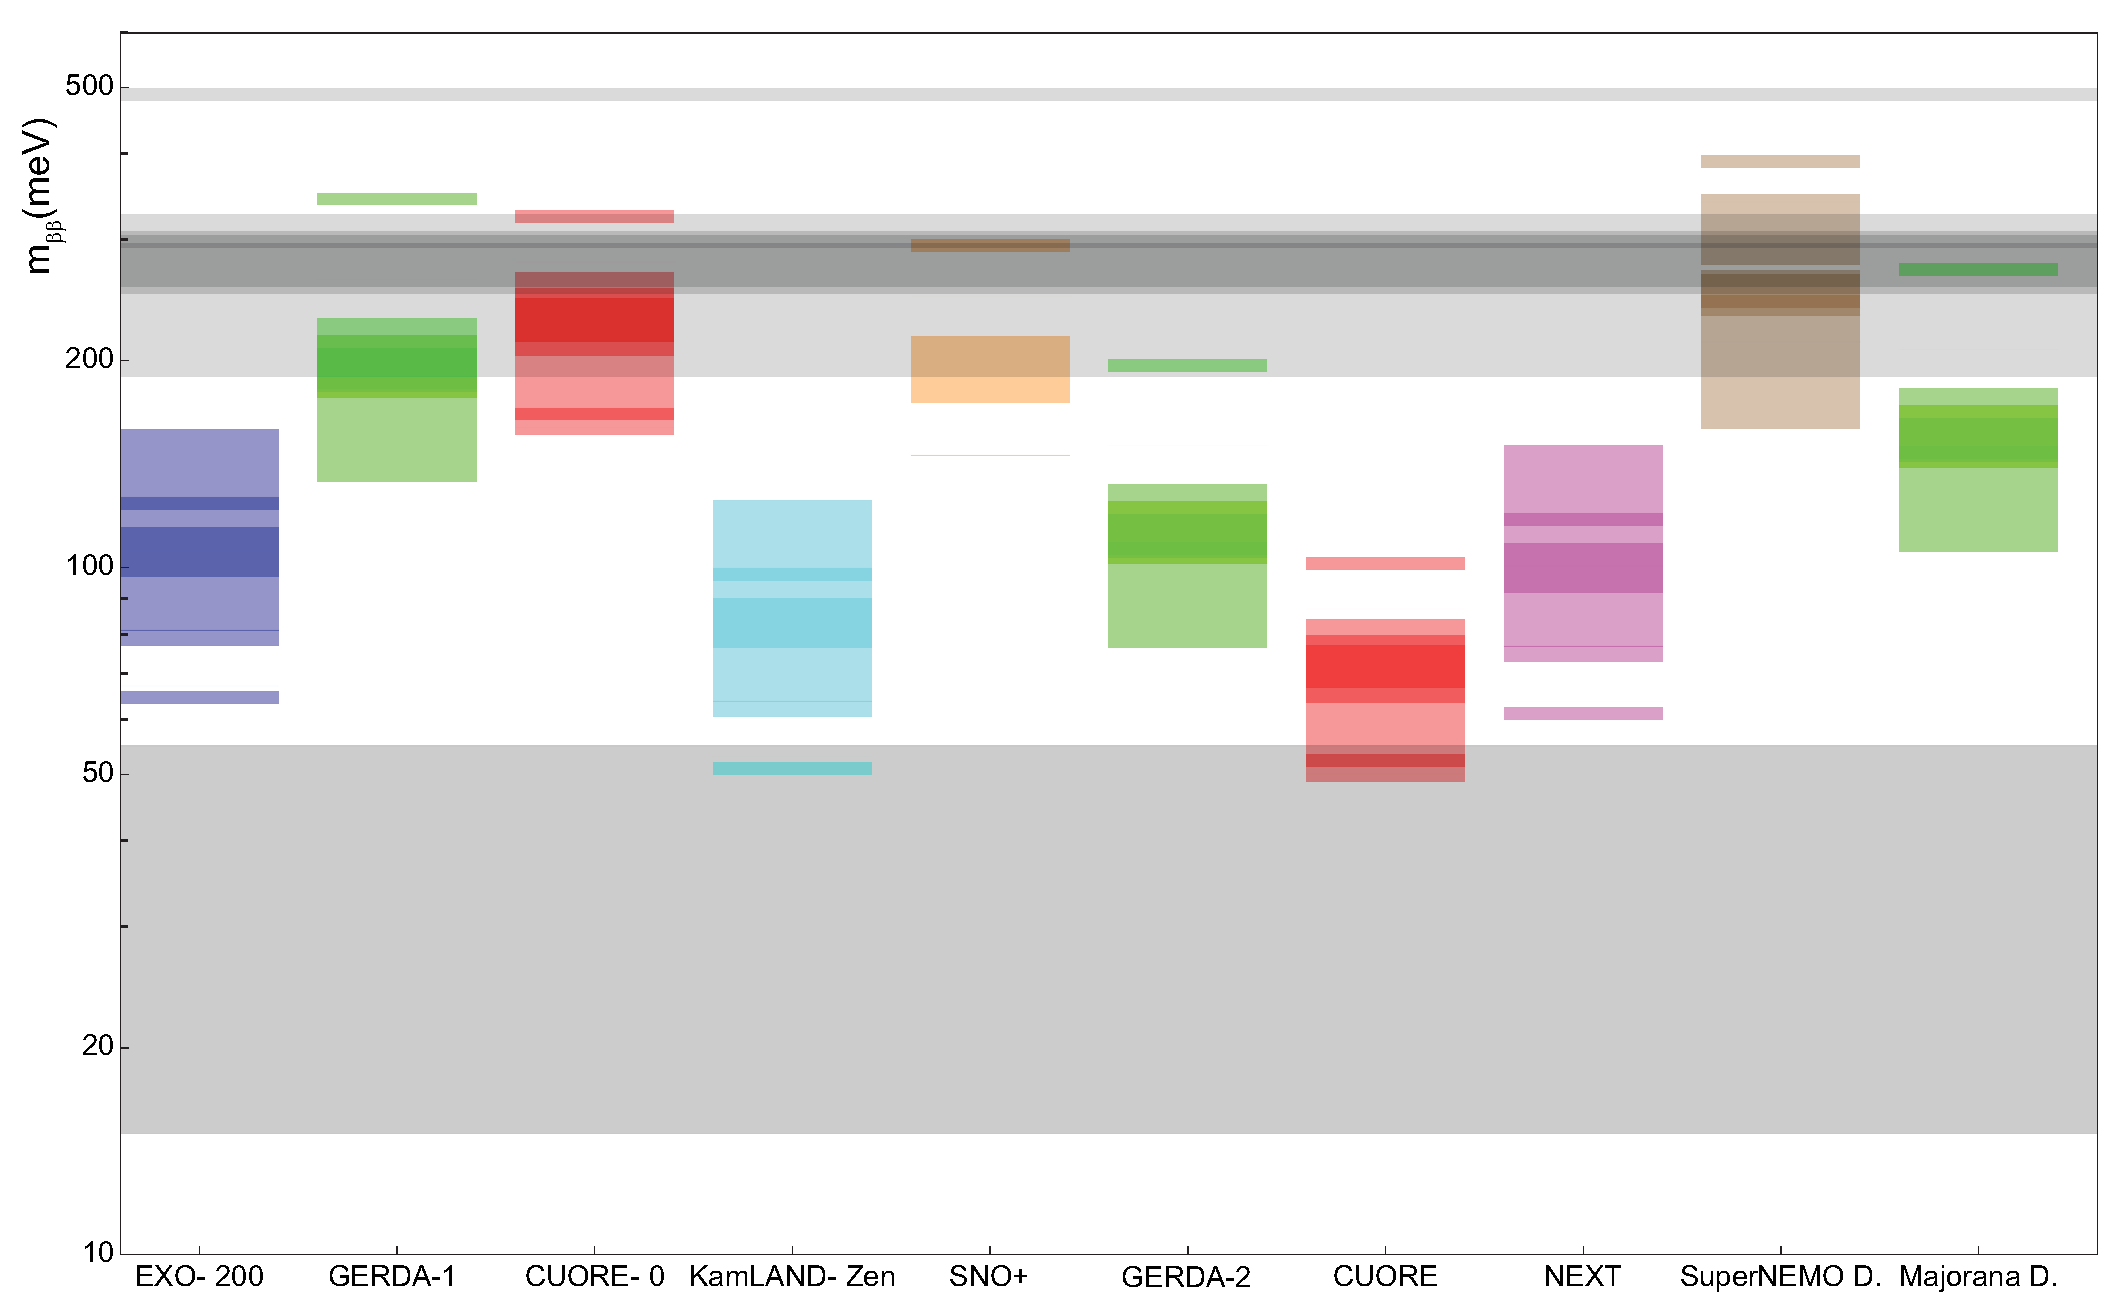
\includegraphics[width=\textwidth]{img/DB_models.eps}
\caption{Sensitivity of the different experiments to the neutrino effective mass \mbb\ computed assuming the optimistic experimental parameters of table~\ref{tab:parameters}. A statistical 90\% CL is computed according to the Feldman-Cousins method \cite{Feldman:1997qc}, assuming a signal region of one FWHM and the corresponding efficiency. Five different frameworks for NME calculations are considered, following reference \cite{Dueck:2011hu}, and are drawn as overlapping rectangles. The upper grey region represents the KK claim \cite{Klapdor-Kleingrothaus:2006zcr} while the lower grey region represents the inverted hierarchy region (see fig.~\ref{fig:mbetabetavsmlight}).}
\label{fig:sens-models}
\end{figure}

Figure~\ref{fig:sens-pmr} represents our main result for the physics case comparison of new-generation \bbonu\ experiments. In this figure, a single, physics-motivated, NME uncertainty band is used for each isotope, following our discussion in sect.~\ref{subsec:nme_pmr}. For completeness, we have also repeated the same exercise for several other NME values or ranges, one for each theoretical framework considered in \cite{Dueck:2011hu}. The result is shown in fig.~\ref{fig:sens-models}. As mentioned above, the spread of the corresponding \mbb\ predictions most likely overestimates the theoretical uncertainty in the \Tonu\ $\to$ \mbb\ sensitivity conversion. For figure clarity, only nuclear theory assumptions are varied in fig.~\ref{fig:sens-models}, while the detector performance parameters are fixed to the most optimistic values of tab.~\ref{tab:parameters}. As can be seen in fig.~\ref{fig:sens-pmr}, our assumed uncertainties in the detector performance parameters would yield \mbb\ sensitivity changes of about the same size as the nuclear theory variations shown in fig.~\ref{fig:sens-models}.


% \subsection{Validity of sensitivity assumptions} \label{subsec:sensi_assumptions}
% The reliability of the sensitivity estimates given above critically depend on how realistic our choice of detector performance indicators is. In this section, we discuss how we have chosen the parameters reported in tab.~\ref{tab:parameters}. This discussion is mostly intended for the expert reader wishing to independently assess our choices, and to use his/her own judgment to modify them accordingly. Given that the largest uncertainty affecting the ultimate \mbb\ sensitivity of a proposal is almost always related the achievable background rates, we decide to quote a background rate range. For all other indicators, a single number rather than a range is used, see tab.~\ref{tab:parameters} 

The EXO-200 TPC is filled with about 175 kg of liquid xenon enriched to 80.6\% in the isotope \XE\ \cite{EXO-200:2011xzf}, corresponding to a \bb\ mass of about 141 \kgbb. For the \bbonu\ efficiency around \Qbb, we take the efficiency assumed by the EXO Collaboration for their \bbtnu\ analysis \cite{EXO-200:2011xzf}, corresponding to $\varepsilon = 0.34$ above the 720 keV analysis threshold. The inefficiencies are dominated by the fiducial volume cut, keeping 63 out of 175 kg of liquid xenon \cite{EXO-200:2011xzf} (0.36 efficiency). A 6.3\% inefficiency introduced by vetoing $\beta$-$\alpha$ coincidences \cite{EXO-200:2011xzf} has also been considered in our efficiency assumption. In \cite{EXO-200:2011xzf}, the collaboration measured an energy resolution of $\sigma_E/E=4.5\%$ at 2615 keV for the EXO-200 detector. This value was obtained using a 376 V/cm drift field and ionization signals only. An improvement of up to a factor of 2.5 could be achieved with higher (1--4 kV/cm) drift fields and combining ionization with scintillation information, see \cite{EXO-200:2003bso}. As a result, we assume a nearly-nominal, 4.2\% FWHM energy resolution at \Qbb, corresponding to about 100 keV. For our background rate lower limit, we consider the collaboration's goal of 20 radioactive background events per year in a $\pm 2\sigma$ interval around the \Qbb\ endpoint, for a $\sigma/E=1.6\%$ energy resolution at 2.5 MeV, a detector mass of 200 kg and a 80\% enrichment in \XE\ \cite{Hall:2010zzg}. From these numbers, we obtain a background rate of $c=0.78\times 10^{-3}$ \ckkbby. This nominal background rate prediction still remains to be updated based on real EXO-200 data. As a worst-case background rate scenario, we take the rate that has already been achieved: $4\times 10^{-3}$ \ckky, see \cite{EXO-200:2011xzf}. This background level was obtained without full lead shielding, radon exclusion tent, radon trap or full 3-dim reconstruction, and might therefore be improved in the future \cite{EXO-200:2011xzf}. This number corresponds to $c=5\times 10^{-3}$ \ckkbby\ per unit \bb\ mass.

GERDA-1 will use eight refurbished \GE\ diodes from the Heidelberg-Moscow and IGEX experiments, for a total active mass of 17.66 kg and 0.86 isotopic enrichment in \GE\ \cite{Knopfle:2012zz}, corresponding to a \bb\ mass of 15.2 \kgbb. As for the \bbonu\ efficiency, the actual value will ultimately depend on analysis details that are unknown at the moment, for example whether the collaboration will rely on pulse shape discrimination already in phase I to further reduce multi-site energy deposition events. In the absence of an updated number, we assume $\varepsilon =0.95$ as originally quoted by the collaboration in \cite{Abt:2004yk}. The FWHM energy resolution for GERDA-1 diodes was measured to be between 3.6 and 6.0 keV at the 2615 keV gamma ray line from \TL\ \cite{Cattadori:2012fy}. Taking the central value of this interval (4.8 keV) and extrapolating to the \GE\ \Qbb\ value (2.039 MeV), we estimate $\Delta E= 4.2\ \text{keV}$. The optimistic background rate scenario is assumed to be the collaboration's goal of 0.01 \ckky\ \cite{Abt:2004yk}, corresponding to 0.012 \ckkbby\ per unit \bb\ mass. GERDA started commissioning in mid-2010, and data obtained since then can be used to estimate a worst-case scenario for the achievable background rates. The best background rate measured with a string of 3 natural germanium detectors, refurbished from the Genius-TF experiment, is $0.06\pm 0.02$ \ckky\ \cite{Cattadori:2012fy}. Since mid-2011, the first enriched germanium detectors have been deployed on a second string arm, using the best detector configuration found so far. Preliminary data from the enriched germanium detectors indicate a background rate that is compatible with the one found with the natural germanium diodes \cite{Cattadori:2012fy}. As a consequence, we assume 0.06 \ckky\ as upper limit for the GERDA-1 background rate, translating into $c=0.07$ \ckkbby\ per unit \bb\ mass.

For the phase II of the experiment, the GERDA Collaboration purchased 37.5 kg of germanium with an isotopic abundance in \GE\ of 0.86. The material has already been purified into 35.4 kg of 6N germanium, corresponding to a \bb\ mass of 30.4 \kgbb. In order to reduce backgrounds, both sophisticated pulse-shape discrimination (PSD) techniques and additional instrumentation for the LAr veto are likely to be used by GERDA-2. We assume an overall \bbonu\ efficiency of $\varepsilon =0.84$, given by the product of the 0.86 efficiency for a PSD cut reported in \cite{Agostini:2010rd}, times the 0.973 efficiency for a LAr veto cut reported in \cite{heisel2011large}. Compared to phase I detectors, a significantly improved FWHM energy resolution of 2 keV at \Qbb\ has been measured for the BEGe detectors to be used by GERDA-2, see \cite{Agostini:2010ke}. The lower limit on the background rate is taken to be the collaboration's goal of 0.001 \ckky\ \cite{Abt:2004yk}, corresponding to $c=0.0012$ \ckkbby. Again, we use preliminary results from the GERDA commissioning runs to estimate an upper limit on the background rate. Commissioning data indicate that $\beta$ decays of $^{42}$K, that is in turn produced positively charged by the $^{42}$Ar decay within the LAr veto, can contribute very significantly to the \Qbb\ background rate. This $^{42}$K background can be most easily quantified by measuring the 1525 keV gamma ray line. On the one hand, the collaboration estimated via simulations that a background rate at \Qbb\ of up to $1.7\times 10^{-3}$ \ckky\ can be obtained by a homogeneous distribution of $^{42}$K around the detectors, for a 43.9 $\mu\text{Bq/kg}$ contamination in $^{42}$K \cite{lehnert2011analysis}. On the other hand, a 1525 keV line about 20 times more intense than expected was observed during the first commissioning run. A significant fraction of this enhancement has been understood as due to a inhomogeneous $^{42}$K distribution caused by the field lines drifting the positively-charged $^{42}$K ions to the detector surface. To prevent the $^{42}$K ions to reach the detector surfaces, the collaboration deployed a copper shield called the \emph{``mini-shroud''}. The additional shroud reduced the counts at the 1525 keV line and at \Qbb\ by a factor of 4-5, and a preliminary measurement of the $^{42}$Ar specific activity of about 160 $\mu\text{Bq/kg}$ was obtained for almost field-free runs \cite{Knopfle:2012zz}. This measured value, combined with the simulation result of $1.7\times 10^{-3}$ \ckky\ for a 43.9 $\mu\text{Bq/kg}$ contamination in $^{42}$K, motivates our upper limit background rate assumption of about 0.006 \ckky, or $c=0.007$ \ckkbby\ per unit \bb\ mass.

CUORE-0 will make use of a single CUORE-like tower with 39 kg of natural TeO$_2$ crystals and with an isotopic abundance of 0.34167 of \TE\ \cite{CUORE:2011boi}, corresponding to a \bb\ mass of 10.9 \kgbb. The overall signal efficiency has been estimated to be about $0.83$, as obtained for the big crystals of the CUORICINO experiment \cite{Andreotti:2010vj}. The main inefficiency source is the ``physical'' inefficiency due to beta particles escaping the detector and radiative processes. The expected FWHM energy resolution of the CUORE detectors is $\Delta E\simeq 5\ \text{keV}$ at the \bbonu\ transition energy \cite{CUORE:2011boi}. As lower limit on the background rate, we assume 0.05 \ckky\ from the 2.615 keV gamma ray multi-Compton events coming from the irreducible \THORIUM\ contamination of the CUORICINO cryostat, as done in \cite{CUORE:2011boi}. This rate corresponds to $c=0.18$ \ckkbby\ per unit \bb\ mass. As upper limit on the background rate, again we follow \cite{CUORE:2011boi} and assume 0.11 \ckky, translating into $c=0.39$ \ckkbby\ per unit \bb\ mass. This latter number includes an additional background contribution from scaling the CUORICINO background in the conservative case of a factor of 2 improvement in \URANIUM\ and \THORIUM\ contamination of the copper and crystal surfaces. Such surface contamination results in degraded alphas that may mimic the \bb\ signal. This factor of 2 improvement is largely motivated by the background rates measured in the Three Towers Test (TTT), allowing to estimate the surface contamination of the copper detector holders, responsible for a large ($50\pm 20\%$ \cite{CUORE:2011boi}) fraction of the CUORICINO backgrounds \cite{Alessandria:2011vj}. For such tests, crystals were dismounted from the CUORICINO detector, and repolished on the surfaces. Three different types of copper cleaning were tested. The copper treatment procedure selected by the collaboration proved to be able to reduce the copper surface contamination by at least a factor of 2 compared to CUORICINO \cite{CUORE:2011boi,Alessandria:2011vj}.  

The CUORE total active mass will be 741 kg for the 988 envisaged cubic detectors \cite{CUORE:2011boi}. As for CUORE-0, the natural TeO$_2$ crystals will have an isotopic abundance of 0.34167 of \TE\ \cite{CUORE:2011boi}, resulting in about 206 \kgbb\ of \TE. The overall signal efficiency and the FWHM energy resolution at \Qbb\ are assumed to be equal to the CUORE-0 figures given above, $\varepsilon =0.83$ and $\Delta E\simeq 5\ \text{keV}$, respectively. The main improvements in background rate reduction compared to CUORE-0 are assumed to come from a much cleaner cryostat and from the different detector geometry. Under these assumptions, the CUORE background will be dominated by copper and crystal surface contaminations. As lower limit on the background rate, the 0.01 \ckky\ goal of the collaboration is assumed \cite{CUORE:2011boi,CUORE:2003fpg}, corresponding to $c=0.036$ \ckkbby. As upper limit, an extrapolation of the currently available measurements \cite{Alessandria:2011vj} on copper and crystal surface contaminations to the CUORE geometry results in a 0.035 \ckky\ upper limit \cite{Gorla:2012gd}, resulting into $c=0.13$ \ckkbby\ per unit \bb\ mass.  

During the phase I of the experiment, KamLAND-Zen will use 389 kg of xenon \cite{kozlov2011status}, enriched to 0.917 \cite{koga2010kamland} in the isotope \XE, for a \XE\ total mass of 357 \kgbb. Concerning \bbonu\ efficiency, the collaboration will make use of a fiducial volume cut to suppress backgrounds that are external to the mini-balloon, for example due to \URANIUM/\THORIUM\ contaminations in the outer liquid scintillator or the environmental gamma ray background. Depending on the \URANIUM/\THORIUM\ contamination levels of the mini-balloon materials themselves (Nylon film, supporting ropes and pipes), the collaboration is also considering a tighter fiducial volume cut to suppress backgrounds originating from the mini-balloon. In the following, we assume that a fiducial volume definition placed 3~$\sigma_r$ inward with respect to the mini-balloon surface will be used, where $\sigma_r$ is the radial position reconstruction accuracy. Assuming $\sigma_r=\mathrm{12.5~cm}/\sqrt{E\mathrm{(MeV)}}$ \cite{kozlov2011status}, we estimate a corresponding fiducial volume efficiency of 0.61 for the 158 cm radius mini-balloon deployed. No other sources of inefficiency are considered in our estimate. Concerning energy reconstruction, the same performance measured in the previous phase of experiment is expected for KamLAND-Zen, given that the xenon-loaded liquid scintillator within the balloon has the same optical properties (light yield, transparency) as the KamLAND scintillator outside the balloon. An energy resolution of $\sigma_E/E=6.8\%/\sqrt{\textrm{E(MeV)}}$ is assumed \cite{kozlov2011status}, scaling to 250 keV FWHM energy resolution at \Qbb. For the background rate lower limit, we take the latest collaboration's expectations, obtained via simulations. In \cite{kozlov2011status}, 19.5 background events per year are expected. The three largest background sources are expected to be \bbtnu\ events entering the ROI, \BI\ events from the mini-balloon materials, and (to a lesser extent) $^{10}\textrm{C}$ events produced through cosmic muon spallation. Compared to previous estimates \cite{koga2010kamland}, a shorter \bbtnu\ half-life as measured in \cite{EXO-200:2011xzf} is assumed ($T_{1/2}\simeq 2\times 10^{21}$ years), together with a less radiopure mini-balloon (\URANIUM/\THORIUM\ concentrations of $3\times 10^{-12}$ g/g). This estimate results in a background rate of $c=0.22\times 10^{-3}$ \ckkbby. Factors that may potentially result in a higher-than-expected background rate are a non-perfect knowledge of the reconstructed energy spectrum of \bbtnu\ events spilling over the ROI, a higher background contribution from mini-balloon materials, and a worse tagging of \BI\ and $^{10}\textrm{C}$ backgrounds (estimated tagging efficiencies of 66\% and 90\%, respectively). It is, however, rather difficult to quantitatively estimate what a ``pessimistic'' background rate might be observed, at this stage. As in the SNO+ discussion below, we assume (to a large extent in a arbitrary fashion) a 8 times higher-than-expected background rate as upper limit. We note that more information to revisit the KamLAND-Zen background model should become available soon, given that KamLAND-Zen data-taking has started.

The MAJORANA demonstrator will contain 40 kg of germanium, of which at least 20 kg and up to 30 kg will be enriched to 86\% in \GE\ \cite{Majorana:2011vap}. We follow the collaboration's baseline and assume 20 kg of enriched germanium \cite{Wilkerson:2012ga}, corresponding to 17.2 \kgbb\ of \GE. A total \bbonu\ efficiency of 71\% is estimated, accounting for detector granularity, pulse-shape analysis (PSA), single-site time correlation (SSTC) and energy cuts. A 5\% loss due to edge effects and lost bremsstrahlung is also included in this number. We divide by the quoted 84\% efficiency of the energy cut alone to estimate a 85\% efficiency in tab.~\ref{tab:parameters}. For energy reconstruction, the 2 keV FWHM resolution measured at \Qbb\ in BEGe detectors \cite{Agostini:2010ke} is assumed, as for GERDA-2. For the background rate, we assume as lower limit the number quoted by the collaboration: 0.004 counts per year and kg in a 4 keV-wide ROI \cite{Majorana:2011vap}, corresponding to $c=1.2\times 10^{-3}$ \ckkbby. Main backgrounds responsible for this rate are expected to be prompt cosmogenics, and \TL/\BI\ contaminants in the cryostat and in the copper/lead shield. A non-negligible contribution from $^{68}$Ge contaminants in the enriched germanium crystals is also expected. The material purity specifications are extremely challenging, with contaminant goals at the $<0.1 (<0.3)\ \mu\mathrm{Bq/kg}$ level in \TL\ (\BI) for the electroformed copper to be used for detector mounts, cryostat and the inner copper shield, and about one order of magnitude worse for the commercial high-purity copper and lead to be used for the outer shield. Purities within one order of magnitude of such goals have already been demonstrated. We therefore assume a factor of 10 worse background rate than nominal as upper limit: $c=12\times 10^{-3}$ \ckkbby.

The SNO+ experiment will make use of 780 tonnes of liquid scintillator \cite{OKeeffe:2011dex}, with natural neodymium loading at the 0.1\% (w/w) \cite{Wright:2009csa}. Given the 5.6\% isotopic abundance of \ND, this concentration corresponds to 44 \kgbb\ of \bb\ emitter mass. The experiment is expected to have a fiducial volume cut rejecting about 50\% of the active volume \cite{Wright:2009csa}. No other sources of inefficiency are considered in our estimate. For energy reconstruction, we assume a light output of 400 NHit/MeV \cite{Wright:2009csa}, or 1347 NHit at \Qbb, where NHit is the number of PMT hits. This number is highly sensitive to the amount of neodymium concentration, and corresponds to 0.1\% (w/w) loading. Such a light output implies a FWHM resolution of about 220 keV at \Qbb. For the background rate, of the order of 100 background events per kton of liquid scintillator and per year are expected via simulations in a 200 keV energy window around \Qbb\ \cite{Wright:2009csa}. This background level translates into a rate of $c=0.009$ \ckkbby, which we take as lower limit. The three dominant backgrounds are expected to be $^8\textrm{B}$ solar neutrinos, \TL\ decays and \bbtnu\ events. The background level due to $^8\textrm{B}$ solar neutrinos is well-known. The \TL\ background assumes a level of \THORIUM\ impurities at the level measured by the BOREXINO experiment, $8.3\times 10^{-18}$ g/g. The collaboration expects energy reconstruction systematic effects, such as non-gaussian resolution tails, on the shape of the \bbtnu\ energy spectrum near the ROI to affect the sensitivity the most, see for example the study in \cite{Wright:2009csa}. Preliminary studies conducted by the collaboration indicate that a \mbb\ sensitivity within a factor of $5/3$ worse than the purely statistical sensitivity can be preserved including this systematic effect. In the large background approximation, which is valid for the SNO+ experiment, this systematic effect would therefore be equivalent to a background rate increase of up to a factor of $(5/3)^4\simeq 8$, resulting in a background rate upper limit of $c=0.07$ \ckkbby.

The NEXT detector will contain 99.14 kg of pressurized xenon gas in the TPC fiducial volume region, enriched to 0.90 in the isotope \XE\ \cite{NEXT:2011eyk}, corresponding to 89.2 \kgbb\ in \bb\ mass. A \bbonu\ efficiency of 0.25 has been estimated via simulations in \cite{NEXT:2011eyk}, accounting for inefficiencies in reconstructing the \bb\ track, and in imposing energy and topology cuts to suppress backgrounds. Given that the inefficiency introduced by the energy within ROI requirement is separately accounted for in our analysis, we assume an efficiency of $\varepsilon =0.25/0.76=0.33$ in tab.~\ref{tab:parameters}. Preliminary energy reconstruction measurements obtained with a kg-scale prototype yield a 4.6\% FWHM resolution at the 59.4 keV full energy peak for a $^{241}$Am calibration source \cite{NEXT:2011eyk}. This energy resolution extrapolates to 0.72\% FWHM resolution at \Qbb, or about 18 keV. As lower limit on the background rate, we take the collaboration's estimate of $0.2\times 10^{-3}$ \ckkbby, dominated by the \URANIUM/\THORIUM\ contamination of the titanium pressure vessel, conservatively assumed to be at the level of $200\ \mu\text{Bq/kg}$ for each isotope, see \cite{NEXT:2011eyk}. Such radiopurity assumptions are based upon the measured upper limits for the clean titanium used in the LUX cryostat \cite{Hall:2010zz}. As upper limit for the background rate, we take an independent (and more pessimistic) measurement of titanium radiopurity, at the level of $1.2\pm 0.4$ ($0.6\pm 0.3$) mBq/kg for \URANIUM\ (\THORIUM) using the Gator low-background counting facility at LNGS \cite{Baudis:2012bc,Baudis:2011am}. Contaminants in these amounts would translate into a background rate of about $10^{-3}$ \ckkbby\ at \Qbb. Also, the collaboration has started its own radiopurity R\&D campaign at LSC, with the goal of refining these assumptions in the near future.

For SuperNEMO, we assume a 7 kg mass in the isotope \SE, to be installed in the demonstrator module \cite{Shitov:2010nt}. A \bbonu\ efficiency of 0.28 has been estimated for a SuperNEMO module in a detailed study \cite{novella2009experimental}, accounting for acceptance, reconstruction efficiency and event selection efficiency. We assume this number in our estimates, which is in fact quite similar to the collaboration's goal of $\varepsilon =0.30$ \cite{Freshville:2011zz}. Calorimeter R\&D efforts achieved a $7.7\%/\sqrt{\textrm{E(MeV)}}$ FWHM energy resolution using a PVT scintillator directly coupled to a 8 inch, high QE, Hamamatsu PMT, see \cite{Freshville:2011zz}. This energy resolution measurement extrapolates to 4.4\% (or about 130 keV) FWHM at \Qbb. For the background rate, we take $c= 6\times 10^{-3}$ \ckkbby\ as worst-case scenario. This number comes from the preliminary result on the \bbonu\ search in \SE\ with the NEMO-3 detector \cite{simard2011results}: 14 events were observed (in agreement with background expectations) in the [2.6--3.2] MeV energy ROI, after 4.5 years of data-taking and 0.93 \kgbb\ of source foil. The backgrounds are dominated by \BI/\TL\ contamination of the foils (measured to be $530\pm 180\ \mu\mathrm{Bq/kg}$ and $340\pm 50\ \mu\mathrm{Bq/kg}$ in \SE, respectively, see \cite{NEMO:2009ewu}) and radon concentration in the tracking volume ($6.46\pm 0.02\ \mathrm{mBq/m}^3$ for the phase-2 of the experiment, see \cite{NEMO:2009ewu}). As background rate lower limit, we assume a factor of 10 improvement in both \TL/\BI\ radiopurity of the foils and in radon concentration in the tracker: $c=0.6\times 10^{-3}$ \ckkbby.

